% WACV 2024 Paper Template
% based on the CVPR 2023 template (https://media.icml.cc/Conferences/CVPR2023/cvpr2023-author_kit-v1_1-1.zip) with 2-track changes from the WACV 2023 template (https://github.com/wacv-pcs/WACV-2023-Author-Kit)
% based on the CVPR template provided by Ming-Ming Cheng (https://github.com/MCG-NKU/CVPR_Template)
% modified and extended by Stefan Roth (stefan.roth@NOSPAMtu-darmstadt.de)

\documentclass[10pt,twocolumn,letterpaper]{article}

%%%%%%%%% PAPER TYPE  - PLEASE UPDATE FOR FINAL VERSION

\usepackage[T1]{fontenc}    % use 8-bit T1 fonts
%\usepackage[review,algorithms]{wacv}      % To produce the REVIEW version for the algorithms track

\newif\ifnonanonymous
\nonanonymoustrue % comment out to be anonymous

\newif\ifuseappendix
\useappendixtrue % comment out to remove appendix

\ifnonanonymous
%\usepackage{wacv}              % To produce the CAMERA-READY version
\usepackage[pagenumbers]{wacv} % To force page numbers, e.g. for an arXiv version
\else
\usepackage[review,applications]{wacv}      % To produce the REVIEW version for the applications track
\fi



% It is strongly recommended to use hyperref, especially for the review version.
% hyperref with option pagebackref eases the reviewers' job.
% Please disable hyperref *only* if you encounter grave issues, e.g. with the
% file validation for the camera-ready version.
%
% If you comment hyperref and then uncomment it, you should delete
% ReviewTempalte.aux before re-running LaTeX.
% (Or just hit 'q' on the first LaTeX run, let it finish, and you
%  should be clear).
\usepackage[pagebackref,breaklinks,colorlinks]{hyperref}


% Include other packages here, before hyperref.
%\usepackage{stfloats}

\usepackage{graphicx}
\usepackage{amsmath}
\usepackage{amssymb}
\usepackage{booktabs}
\usepackage{comment}
\usepackage{multicol}


\usepackage{url}            % simple URL typesetting
\usepackage{amsfonts}       % blackboard math symbols
\usepackage{nicefrac}       % compact symbols for 1/2, etc.
\usepackage{microtype}      % microtypography
\usepackage{lipsum}         % Can be removed after putting your text content
\usepackage[numbers]{natbib}
\usepackage{doi}

%% extra
\usepackage{listings}
\usepackage{amsmath} 
\usepackage{xcolor}
\usepackage[toc]{appendix}

% Support for easy cross-referencing
\usepackage[capitalize]{cleveref}
\crefname{section}{Sec.}{Secs.}
\Crefname{section}{Section}{Sections}
\Crefname{table}{Table}{Tables}
\crefname{table}{Tab.}{Tabs.}

\newcommand{\cotwo}{\ensuremath{\mathrm{CO_2}}}


%%%%%%%%% PAPER ID  - PLEASE UPDATE
\def\wacvPaperID{*****} % *** Enter the WACV Paper ID here
\def\confName{WACV}
\def\confYear{2025}


\begin{document}

\title{``ScatSpotter'' --- A Distributed Dog Poop Detection Dataset}

\author{Jonathan Crall\\
Kitware\\
{\tt\small jon.crall@kitware.com}
%{\tt\small erotemic@gmail.com}
% For a paper whose authors are all at the same institution,
% omit the following lines up until the closing ``}''.
% Additional authors and addresses can be added with ``\and'',
% just like the second author.
% To save space, use either the email address or home page, not both
%\and
%Second Author\\
%Institution2\\
%First line of institution2 address\\
%{\tt\small secondauthor@i2.org}
}
\maketitle

%%%%%%%%% ABSTRACT
\begin{abstract}

%This work chronicles one researcher's un-funded journey to build a phone
%application that can detect dog poop in images, and make the data widely
%available as a benchmark dataset.
We introduce a new --- currently 42 gigabyte --- "living" dataset of phone images of dog feces, annotated with manually drawn or AI-assisted polygon labels. There are 6k full resolution images and 4k detailed polygon annotations. The collection and annotation of images started in late 2020 and the dataset grows by roughly 1GB a month. 

We train a baseline vision transformer to segment the objects of interest, exploring a grid of hyperparameters, and we evaluate their impact.  The best model achieves a pixelwise average precision of 0.78 on a 691-image validation set and 0.51 on a small independently captured 30-image contributor test set.

The most recent snapshot of dataset is made publicly available through three different distribution methods: one centralized and two decentralized (IPFS and BitTorrent).  We perform an analysis and observational comparison of the trade-offs between distribution methods and discuss the feasibility of each with respect to sharing open scientific data in a reliable and accessible manner.

The code to reproduce the experiments is hosted on GitHub, and the data is published under the Creative Commons Attribution 4.0 International license.  Model weights are made publicly available with the dataset. Experimental hardware, time, energy, and emissions are quantified.

%A phone application to detect poop with these models is being developed and 
%will be made freely available.
\end{abstract}

%%%%%%%%% BODY TEXT
\section{Introduction}
\label{sec:intro}

Applications for a computer vision system capable of detecting and localizing poop in images are numerous.
These include automated waste disposal to keep parks and backyards clean, tools for monitoring wildlife
  populations via droppings, and a warning system in smart-glasses to prevent people from stepping in poop.
Our primary motivating use case is a phone application that assists dog owners in locating their dog's poop
  in a leafy park for easier cleanup.
Many of these applications can be realized with modern object detection and segmentation methods
  \cite{sandler_mobilenetv2_2018, siam_rtseg_2018, yu_mobilenet_yolo_2023} combined with a large labeled
  dataset.

\begin{figure}[ht]
\centering
\includegraphics[width=0.49\textwidth]{figures/zoom_leaf.jpg}
%\hfill
%\includegraphics[width=0.49\textwidth]{figures/Screenshot from 2024-09-07 19-20-25.png}
\caption[]{
    A zoomed in example of an annotated object in a challenging
    condition: a scene cluttered with leafs. Polygons were drawn an AI-assistant,
    which means boundaries are sometimes imperfect.
}
\label{fig:HardCase}
\end{figure}

\begin{figure}[ht]
\centering
\includegraphics[width=0.49\textwidth]{figures/viz_three_images.jpg}
\caption[]{
The "before/after/negative" protocol.
The orange box highlights the location of the poop 
%(note the actual annotation is a polygon)
in the "before" image.
In the "after" image, it is the same scene but the poop has been removed.
The "negative" image is a nearby similar scene, potentially with a distractor.
Note that the object is small relative to the image size.}
\label{fig:ThreeImages}
\end{figure}

\begin{table*}[t]
\begin{tabular}{lrrrcrrl}
\toprule
Name & \#Cats & \#Images & \#Annots & Image W \times H & Annot Area$^{0.5}$ & Size & Annot Type \\
\midrule
ImageNet LSVRC2017 \cite{ILSVRC15} & 1,000 & 594,546 & 695,776 & 500 \times 374 & 239 & 166GB & box \\
MSCOCO 2017 \cite{lin_microsoft_2014} & 80 & 123,287 & 896,782 & 428 \times 640 & 57 & 50GB & polygon \\
CityScapes \cite{cordts2015cityscapes} & 40 & 5,000 & 287,465 & 2,048 \times 1,024 & 50 & 78GB & polygon \\
ZeroWaste \cite{bashkirova_zerowaste_2022} & 4 & 4,503 & 26,766 & 1,920 \times 1,080 & 200 & 10GB & polygon \\
TrashCanV1 \cite{hong2020trashcansemanticallysegmenteddatasetvisual} & 22 & 7,212 & 12,128 & 480 \times 270 & 54 & 0.61GB & polygon \\
UAVVaste \cite{rs13050965} & 1 & 772 & 3,718 & 3,840 \times 2,160 & 55 & 2.9GB & polygon \\
SpotGarbage-GINI \cite{mittal2016spotgarbage} & 1 & 2,512 & 337 & 754 \times 754 & 355 & 1.5GB & classification \\
TACO \cite{proenca_taco_2020} & 60 & 1,500 & 4,784 & 2,448 \times 3,264 & 119 & 17GB & polygon \\
MSHIT \cite{mshit_2020} & 2 & 769 & 2,348 & 960 \times 540 & 99 & 4GB & box \\
``ScatSpotter'' (ours) & 1 & 6,648 & 4,386 & 4,032 \times 3,024 & 96 & 42GB & polygon \\
\bottomrule
\end{tabular}
\caption{Related Datasets.
The first 4 columns provide the name of the dataset, the number of categories, images, and annotations.
Image W \times H is the pixel width and height of the image with the median area. Annot Area$^{0.5}$ is the median sqrt(area) in pixels of the annotation polygon or box. The Size column refers to the amount of information in  gigabytes needed to download the entire dataset.
Annot Type refers to if the dataset is annotated with bounding boxes,
image-level classification labels, or polygon segmentations.
%Of the datasets in this table, ours has the highest image resolution
%and the smallest annotation size relative to that resolution.
% Of the waste related datasets, ours is among the largest, and of the poop related datasets, it is the largest.
}
\label{tab:related_datasets}
\end{table*}

In addition to enabling several applications, poop detection is an interesting benchmark problem.
It is relatively simple, with a narrow focus on a single class, making it suitable for exploring the
  capabilities of object detection models that target a single labeled class.
However, the task includes non-trivial challenges such as resolution issues (e.g., camera quality,
  distance), distractors (e.g., leaves, pine cones, sticks, dirt, and mud), occlusion (e.g., bushes, overgrown
  grass), and variation in appearance (e.g., old vs. new, healthy vs. sick).
An example of a challenging case is shown in \cref{fig:HardCase}.
Investigation into cases where this problem is difficult may provide insight
into how to better train object detection and segmentation networks.

Towards these ends we introduce a new dataset, which for the purpose of this paper we call "ScatSpotter".
Poops are annotated with polygons making the dataset suitable for training detection and segmentation
  models.
In order to assist with annotation and add variation, we collect images using a "before/after/negative"
  protocol as shown in \Cref{fig:ThreeImages}.
We train a segmentation model to classify which pixels in an image contain poop and which do not.
Our models show strong performance, but there are notable failure cases indicating this problem is difficult
  even for modern computer vision algorithms.

To enable others to build on our results, it is essential that the dataset is accessible and hosted
  reliably.
Centralized methods are a typical choice, offering high speeds, but they can be costly for individuals,
  often requiring institutional support or paid hosting services.
They are also prone to outages and lack built-in data validation.
In contrast, decentralized methods allow volunteers to host data and offers built-in validation of data
  integrity.
This motivates us to compare and contrast the decentralized BitTorrent \cite{cohen_incentives_2003}, and
  IPFS \cite{benet_ipfs_2014} protocols as mechanisms for distributing datasets.

% VGG2 face got removed.
% https://github.com/ox-vgg/vgg_face2/issues/52

Our contributions are:
1) A challenging new \textbf{open dataset} of images with polygon annotations.
2) An experimental \textbf{evaluation of baseline training} methods.
3) An observational \textbf{comparison of dataset distribution} methods.
4) \textbf{Open code and models}.

%\Cref{sec:dataset}.
%\Cref{sec:models}.
%\Cref{sec:distribution}.
%\Cref{sec:relatedwork}.


%-------------------------------------------------------------------------
\section{Related Work}
\label{sec:relatedwork}

To the best of our knowledge, our dataset is currently the largest publicly available collection of
  annotated dog poop images, but it is not the first.
A dataset of 100 dog poop images was collected and used to train a FasterRCNN model
  \cite{neeraj_madan_dog_2019} but this dataset and model are not publicly available.
The company iRobot has a dataset of annotated indoor poop images used to train Roomba j7+ to avoid
  collisions \cite{roomba_2021}, but as far as we are aware, this is not available.
In terms of available poop detection datasets we are only aware of MSHIT~\cite{mshit_2020} which is much
  smaller, only contains box annotations, and the objects of interest are plastic toy poops.

Compared to benchmark object localization and segmentation datasets~\cite{ILSVRC15,
  lin_microsoft_2014,cordts2015cityscapes} ours is much smaller and focused only on a single category.
However, when compared to litter and trash datasets
  \cite{bashkirova_zerowaste_2022,proenca_taco_2020,hong2020trashcansemanticallysegmenteddatasetvisual,mittal2016spotgarbage,rs13050965}
  ours is among the largest in terms of number of images / annotations, image size, and total dataset size.
ZeroWaste~\cite{bashkirova_zerowaste_2022} uses a "before/after" protocol similar to our BAN-protocol.
%% https://paperswithcode.com/dataset/taco
We provide an overview of these related datasets in \Cref{tab:related_datasets}.
Among all of these, ours stands out for having the highest resolution images and the smallest objects
  relative to that resolution.
For a review of additional waste related datasets, refer to \cite{agnieszka_waste}.
%Additional waste-related datasets not discussed here are reviewed in \cite{agnieszka_waste}.

%There are also smaller waste detection related datasets.
%%Waste detection is an important problem but with relatively few open datasets.
%%  https://paperswithcode.com/dataset/zerowaste
%ZeroWaste \cite{bashkirova_zerowaste_2022} (9.9GB) contains 1,800 segmented video frames and
%  6,000 unlabeled frames in a recycling facility, and they also use a similar "before/after" protocol.
%% https://paperswithcode.com/dataset/taco
%TACO \cite{proenca_taco_2020} (17GB) is another "living" dataset containing 1,500 images with
%  4,784 polygon annotations over 60 classes.
% TrashCan https://paperswithcode.com/dataset/trashcan
% Top Datasets on paperwith code
% https://paperswithcode.com/datasets?mod=images&task=semantic-segmentation&page=2


% Domestic Trash / Garbage Dataset
% Looks like the full dataset is behind a paywall
% https://paperswithcode.com/dataset/domestic-trash-garbage-dataset


% https://universe.roboflow.com/dataset-vmyna/poop-yxidr/dataset/1
% 102 train images, 22 validation images, 0 test images.
% human poop
In \Cref{sec:distribution} will discuss the logistics and tradeoffs between different mechanisms to
  distribute datasets with a focus on comparing centralized and decentralized methods.
IPFS~\cite{cohen_incentives_2003} and BitTorrent~\cite{benet_ipfs_2014} are the decentralized distribution
  mechanism we evaluate, but there are others such as Secure Scuttlebut \cite{tarr_secure_2019} and Hypercore
  \cite{frazee_dep-0002_nodate}, which we did not test.

  % Is hypercore dat? https://dat-ecosystem.org/ https://datproject.org/

% Very good overview and comparison of the protocols
% https://blog.mauve.moe/posts/protocol-comparisons
% https://distributed.press/
% hypercore - https://github.com/tradle/why-hypercore/blob/master/FAQ.md#how-is-hypercore-different-from-ipfs
% git,
% Secure Scuttlebut (SSB)

\section{Dataset}
\label{sec:dataset}

Our first contribution is the creation of a new open dataset which consists of images of dog poop in mostly
  urban, mostly outdoor environments.
The data is annotated to support object detection and segmentation tasks.
The majority of the images feature fresh poop from three specific dogs, but there are a significant number
  of images with poops of unknown age and from from unknown dogs.


More details about the dataset are available in a standardized datasheet
\cite{gebru_datasheets_2021} that covers the motivation, composition,
collection, preprocessing, uses, distribution, and maintenance. This will be
distributed with the data itself, and is provided in supplemental material.

\subsection{Dataset Collection}

The dataset was primarily collected by a single researcher while walking their dogs.
When they encountered a poop in public areas --- usually freshly created by one of their own dogs, but
  sometimes from other dogs --- they would take an image of the poop from their original vantage point.
Occasionally, they would move closer or further away to add variation to the dataset.
After taking a photo, they would pick it up and dispose of it.

Most images in the dataset follow a "before/after/negative" (B/A/N) protocol.
The first image is the "before" picture of the poop.
After picking up the poop, an "after" picture of the same area was taken from approximately the same angle
  and distance.
Finally, a "negative" image was captured of a nearby area or object that might be confused with dog poop
  (e.g., pine cones, leaves, sticks, dark areas on snow).
While we only use these B/A/N triples to sample negative regions, they may be useful for constructing
  contrastive triplet-style losses \cite{schroff_facenet_2015}.

The majority of images follow the triple-pattern protocol.
However, there are exceptions.
The first six months of data collection only involved the "before/after" part of the protocol, and we began
  collecting the third negative image after a colleague suggested it.
In some cases, the researcher failed or was unable to take the second or third image.
These exceptions were programmatically identified.
  
In addition to the primary dataset, we also received 84 images from contributors.
Most of these images do not follow the B/A/N protocol and are marked for use only in testing and are
  \emph{not} included in the following analysis unless explicitly noted.


\subsection{Dataset Annotation}

Originally the "before" and "after" images were meant to help with automatic
annotation, but this idea was not successful due to unreliable image-alignment.
However, with the development of the Segment Anything Model (SAM)
\cite{kirillov_segment_2023} model, we were able to efficiently annotation the
dataset. 

Specifically, images were annotated using labelme \cite{wada_labelmeailabelme_nodate}. 
Most annotations were initialized using the SAM and a point prompt. 
All AI polygons were manually reviewed. In most cases only small manual
adjustments were needed, but there were a significant number of cases where SAM
did not work well and fully manual annotations were needed.
Regions with shadows seemed to cause SAM the most trouble, but there were other
failure cases. Unfortunately, there is no metadata to indicate which polygons
were manually created or done using AI.  However, the number of vertices may be
a reasonable proxy to estimate this, as polygons generated by SAM tend to have
higher fidelity boundaries.  The boundaries of 4,386 annotated polygons are
illustrated in \Cref{fig:AllPolygons}.

%Anecdotal note: SAM \cite{kirillov_segment_2023} worked well to automatically
%segment the poop, many of these needed adjustments, especially in regions of
%shadows, but there were cases that required a completely manual approach.
%Unfortunately a clean record of what cases these were does not exist. 

\begin{figure}[ht]
\centering
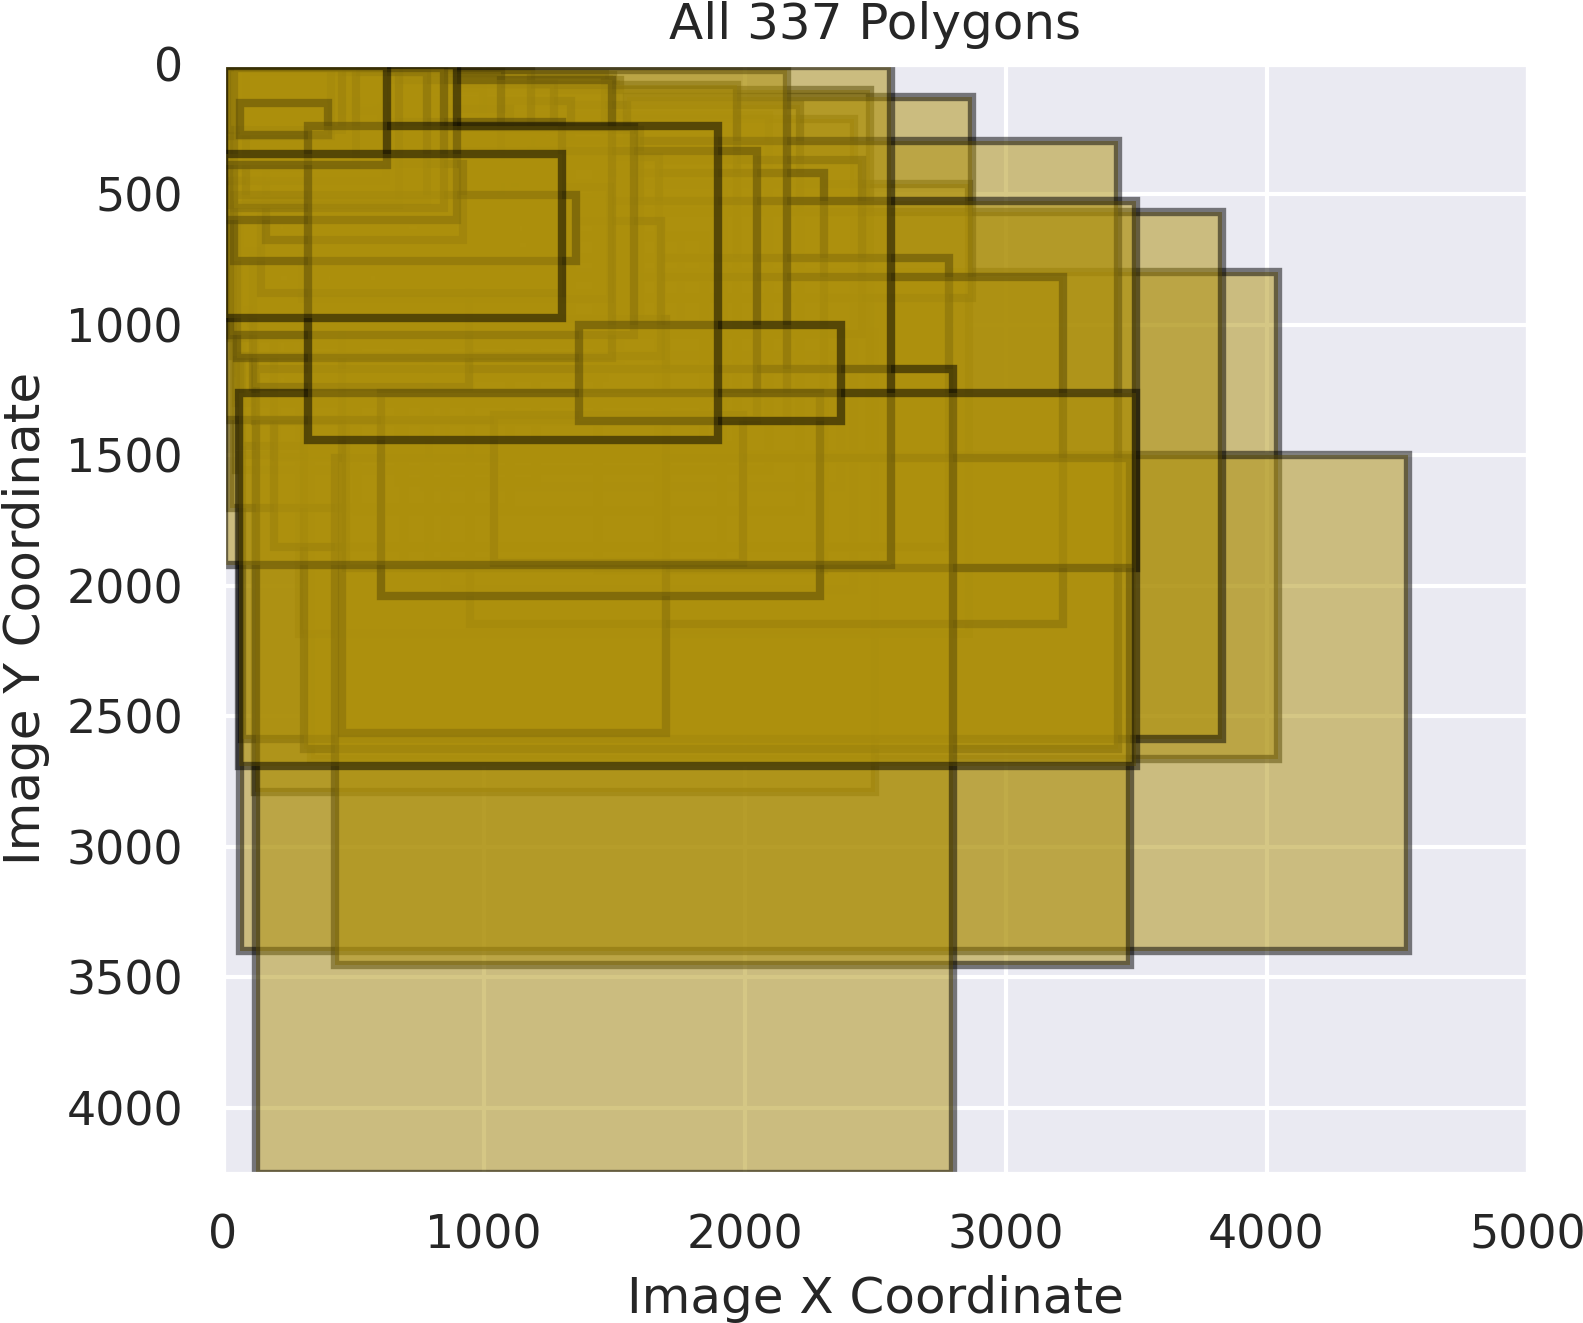
\includegraphics[width=0.4\textwidth]{figures/all_polygons.png}
\caption[]{
    All polygon annotations drawn in a single plot with 0.8 opacity to
    demonstrate the distribution in annotation location, shape, and size with
    respect to image coordinates. Annotations drawn with AI
    assistance tend to have more curved boundaries than manually drawn ones
    (several examples of manual annotations with more jagged boundaries can be
    seen in the top left).
}
\label{fig:AllPolygons}
\end{figure}

\begin{figure}[ht]
\centering
\includegraphics[width=0.4\textwidth]{figures/images_timeofday_distribution.png}
\caption[]{
    Scatterplot of the time-of-year vs time-of-day each image was taken.
    On the x-axis, 0 is January 1st.
    On the y-axis, 0 is midnight.
    For images with geolocation and timestamp (assuming the timezone is local or given and correct) we also
      estimate the amount of daylight as indicated by the color of each dot.
    While the majority of the images are taken in daylight, there are a sizable number of nighttime images taken with longer exposure, flash on, or sometimes flash off in streetlights.
}
\label{fig:TimeOfDayDistribution}
\end{figure}


\begin{figure}[ht]
\centering
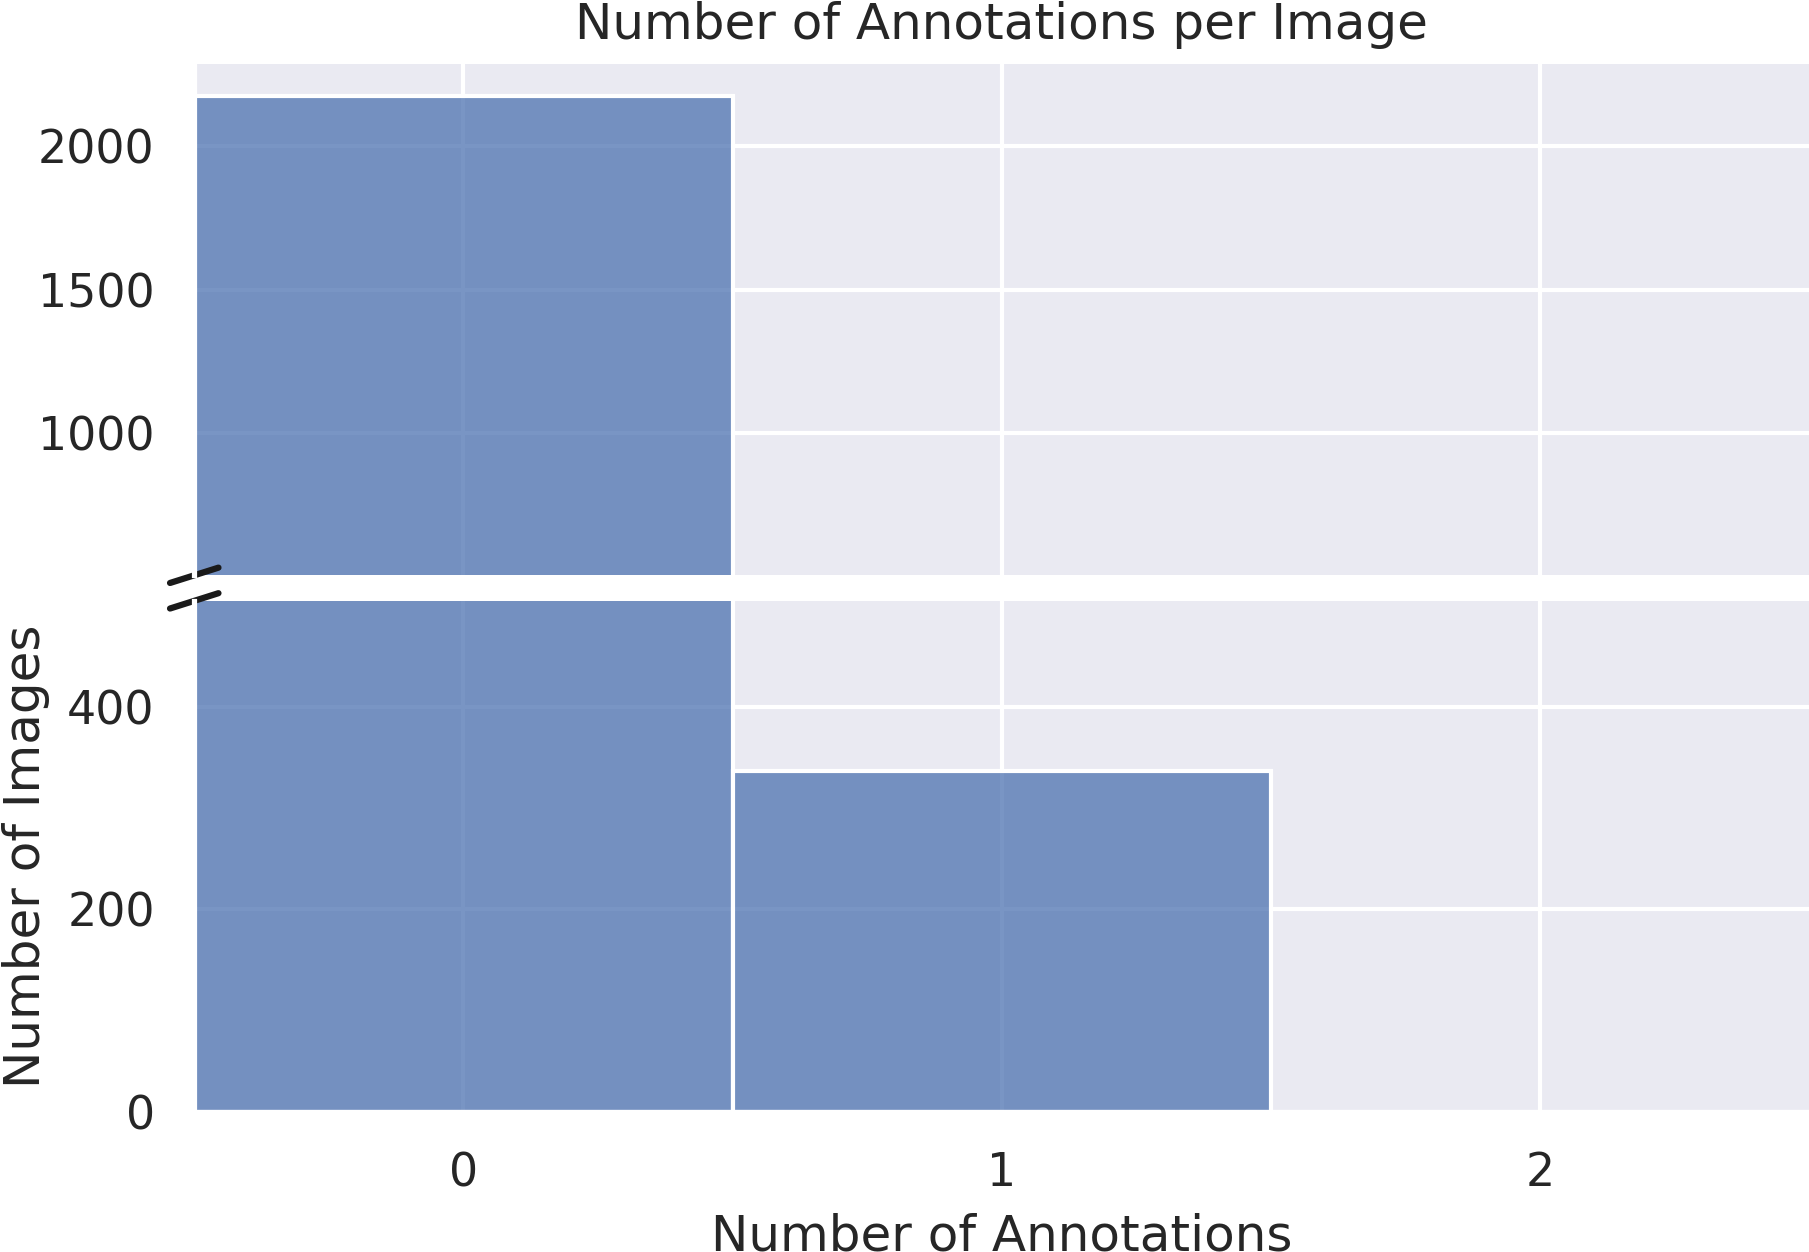
\includegraphics[width=0.4\textwidth]{figures/anns_per_image_histogram_splity.png}
\caption[]{
    Histogram of the number of annotations per image. 
    Only 35\% (2,346) of the images contain annotations, the other 65\% (4,302)
    are known not to contain poop. Of these 4,302 about half of them were taken
    directly after the poop was picked up, and the other half are pictures of a
    nearby location.
}
\label{fig:AnnotsPerImage}
\end{figure}


\subsection{Dataset Stats and Analysis}

% Number of images, annotations, and other stats.
As of 2024-07-03, the primary dataset consists of 6,648 images and 4,386 annotations, spanning 3.5 years.
The data was captured at a relatively uniform rate over this period, primarily in parks and sidewalks within
  a small city.
Weather conditions varied across snowy, sunny, rainy, and foggy.
A visual representation of the distribution of seasons, time-of-day, daylight, and capture rate is provided
  in \Cref{fig:TimeOfDayDistribution}.


The dataset images are available in full resolution, without any resampling or resizing.
Almost all images were taken using the same phone-camera, with a consistent width/height ratio of 4,032
  $\times$ 3,024 (although some may be rotated based on EXIF data).
Six images have a slightly different resolution of 4,008 $\times$ 5,344, and one has a resolution of 7,680
  $\times$ 1,024.
The images are stored as 8-bit JPEGs with RGB channels, and most include overviews (i.e., image pyramids),
  allowing for fast loading of downscaled versions.


Due to the "B/A/N" protocol, approximately one-third of the dataset contains annotations, as the other
  two-thirds of images were taken after removing the object of interest from the scene.
Consequently, most images have no annotations.
The next most frequent number of annotations is one, but images can contain multiple annotations due to
  several reasons:
1) A single poop may break into multiple disjoint parts (although the exact criteria for this can be
  ambiguous).
2) Two dogs may have pooped nearby each other.
3) One or more dogs may have pooped in the same area over a period of time (in some cases, it can be
  challenging to determine if it is poop or dirt).
The number of annotations per image is illustrated in \Cref{fig:AnnotsPerImage}.


\subsection{Dataset Splits}

Our dataset is split into training, validation, and test sets based on the year and day of image capture.
Specifically, images from 2021, 2022, and 2023 are assigned to the training set, while images from 2020 are
  used for validation.
For data from 2024, we consider the Gregorian ordinal date $n$ of each image and include it in the validation set if
$n \equiv 0 \ (\textrm{mod}\ 3)$; otherwise, it is assigned to the training set.

The resulting splits are as follows:
Our training dataset consists of 5,747 images and is identified by a suffix of {\tt 1e73d54f}, which is the
  prefix of a hash of its contents.
The validation set contains 691 images and has a suffix of {\tt 99b22ad0}.
The test set, consisting of the 30 contributor images with at least one annotation, has a suffix of {\tt
  d8988f8c}.
These splits are provided in the COCO JSON format \cite{lin_microsoft_2014}.


\section{Models}
\label{sec:models}

As our second contribution, we evaluate several trained models to establish a baseline for future
  comparisons.
We use the training, prediction, and evaluation system presented in \cite{Greenwell_2024_WACV,
  crall_geowatch_2024}, which utilizes polygon annotations to train a pixelwise binary segmentation model.
%It is important to note that this baseline is limited in that it only considers a single VIT-based
%  \cite{dosovitskiy_image_2021} architecture, and does not attempt to explore all state-of-the-art methods.


In all experiments, we use half-resolution images, which means most images have an effective width $\times$
  height of 2,016 $\times$ 1,512.
We employ a spatial window size of 416 $\times$ 416 for network inputs, which means that multiple windows
  are needed to predict on entire images.
During prediction, we apply a window overlap of 0.3 with feathered stitching to prevent boundary artifacts.

To address the class imbalance in our dataset (where positives are patches containing annotations and
  negatives contain no annotations), we adopt a balanced sampling strategy.
Each "epoch" consists of randomly sampling 32,768 patches from the dataset with replacement, ensuring
  roughly equal numbers of positive and negative samples.
We train each network for 163,840 gradient steps.
For data augmentation we use random crops and flips.

Our baseline architecture is a variant \cite{bertasius2021space,Greenwell_2024_WACV} of a vision-transformer
  \cite{dosovitskiy_image_2021}.
The model is a 12-layer encoder backbone with 384 channels and 8 attention heads that feeds into a 4-layer
  MLP segmentation head.
It has 25,543,369 parameters and a size of 114.19 MB on disk.
At predict time it uses 1.96GB of GPU RAM.

We compute loss pixelwise using Focal Loss \cite{ross2017focal} with a small downweighting of pixels towards
  the edge of the window.
Our optimizer is AdamW \cite{loshchilov_decoupled_2018}, and we experiment with varying learning rate,
  weight decay, and perturb-scale (implementing the shrink perturb trick~\cite{ash_warm_starting_2020,dohare_loss_2023}).
We employ a OneCycle learning rate scheduler \cite{smith2019super} with a cosine annealing strategy and
  starting fraction of 0.3.
Our effective batch size is 24 with a real batch size of 2 and 12 accumulate gradient steps.
This setup consumes approximately 20 GB of GPU RAM during training.
  

\subsection{Model Experiments}

%In order to find a strong baseline we evaluated 35 different hyperparamter training runs over different
%  input resolutions, window sizes, model depth, and other parameters in a somewhat ad-hoc manner.
%Taking the best hyperparameters from that search, we perform a sweep over 7 combinations of learning rate,
%  weight decay, and perterb scale (i.e.
%shrink and perterb \cite{ash_warm_starting_2020}).
%Scripts to reproduce these experiments as well as a log of the ad-hoc experiments are in the code repo.
%Models are also distributed with information about how they were trained.
%using stochastic engineer descent.

To establish a strong baseline, we evaluated 35 training runs where we varied input resolutions, window
  sizes, model depth, and other parameters.
Although this initial search was somewhat ad-hoc, it provided insights into the optimal configuration for
  our model.
Building on the best hyperparameters from this search, we performed a sweep over 7 combinations of learning
  rate, weight decay, and perturb scale (i.e., shrink and perturb \cite{ash_warm_starting_2020,dohare_loss_2023}).
Scripts used to reproduce these experiments, as well as a log of the ad-hoc experiments, are available in
  the code repository.
Additionally, trained models are packaged and distributed with information about their training
  configuration.


\begin{table*}[t]
\centering
\begin{tabular}{llllllll}
\toprule
            \multicolumn{4}{l}{} & \multicolumn{2}{c}{validation} & \multicolumn{2}{c}{test} \\
config name &   lr & weight\_decay & perterb\_scale & AP & AUC & AP & AUC \\
\midrule
        \textcolor[HTML]{623682}{D05} & 1e-4 &   1e-6 &  3e-6 & \textbf{0.7802} & \textbf{0.9943} &          0.5051 &          0.9125 \\
        \textcolor[HTML]{df8020}{D03} & 1e-4 &   1e-5 &  3e-7 &          0.7758 &          0.9707 &          0.4346 &          0.8576 \\
        \textcolor[HTML]{87b787}{D04} & 1e-4 &   1e-7 &  3e-7 &          0.7725 &          0.9818 &          0.4652 &          0.7965 \\
        \textcolor[HTML]{207fdf}{D02} & 1e-4 &   1e-6 &  3e-7 &          0.7621 &          0.9893 & \textbf{0.5167} & \textbf{0.9252} \\
        \textcolor[HTML]{20df20}{D00} & 3e-4 &   3e-6 &  9e-7 &          0.7571 &          0.9737 &          0.4210 &          0.7766 \\
        \textcolor[HTML]{df20df}{D01} & 1e-3 &   1e-5 &  3e-6 &          0.7070 &          0.9913 &          0.4607 &          0.9062 \\
        \textcolor[HTML]{b00403}{D06} & 1e-4 &   1e-6 &  3e-8 &          0.6800 &          0.9773 &          0.4137 &          0.8157 \\
        
\bottomrule
\end{tabular}
\caption{
%Scores for the best top model on the validation set for each of the 7 hyperparameter configurations.
%These correspond to the maximum AP of each run in \Cref{fig:apauc_scatter}.
%The first column (config name) provides the code for a particular training run used in the score scatter
%  and box plots.
%The next three columns correspond to the value of the varied hyperparameters that run.
%Then the AP and AUC scores on the validation set are given.
%The final two columns are the AP and AUC scores on the test set for these same validation-maximizing
%  models models.
%(The top AP score on the test set was 0.65, but it did not correspond to one of these validation runs
%  used to select models).
%Qualitative examples on the test, validation, and training set are given in
%  \cref{fig:test_heatmaps_with_best_vali_model} all on the top-scoring validation model listed here.
Results for the best-performing models on the validation set across 7 hyperparameter configurations.
%These results correspond to the maximum Average Precision (AP) scores shown in \Cref{fig:apauc_scatter}.
The table provides detailed information about each configuration, including:
1) Configuration name (first column): a unique code identifying each training run used in the score scatter and box plots.
2) Varied hyperparameters (next three columns): specific values for learning rate, weight decay, and perturb scale that were used in each run.
3) Validation set performance (AP and AUC scores): metrics evaluating the model's performance on the validation set.
4) Test set performance (AP and AUC scores): metrics evaluating the model's performance on the test set using the same validation-maximizing models.
Note that the top AP score over all models on the test set was 0.65, but it did not correspond to one of these validation runs used for model selection.
Qualitative examples illustrating the performance of the top-scoring validation model listed here are provided in \cref{fig:test_heatmaps_with_best_vali_model}.
%for the test, validation, and training sets.
}
\label{tab:parameters_and_results}
\end{table*}

\begin{comment}
    SeeAlso:
    ~/code/shitspotter/experiments/geowatch-experiments/run_pixel_eval_on_vali_pipeline.sh
    python ~/code/shitspotter/dev/poc/estimate_train_resources.py
\end{comment}

For each of the 7 hyperparameter combinations, we trained the model for 163,840 optimizer steps using a
  batch size of 24.
We defined an "epoch" as 1,365 steps, at which point we saved a checkpoint, evaluated validation loss, and
  adjusted learning rates.
To conserve disk space, we retained only the top 5 lowest-validation-loss checkpoints (although training
  crashes and restarts sometimes resulted in additional checkpoints, which are included in our evaluation).

Using the top-checkpoints, we predicted heatmaps for each image in the validation set.
We then performed binary classification on each pixel (poop-vs-background) using a threshold.
Next, we rasterized the truth polygons.
The corresponding truth and predicted pixels were accumulated into a confusion matrix, allowing us to
  compute standard metrics such as precision, recall, false positive rate, etc.
\cite{powers_evaluation_2011} for the specific threshold.
By sweeping a range of thresholds, we calculated the average precision (AP) and the area under the ROC curve
  (AUC).
We computed all metrics using scikit-learn \cite{scikit-learn}.
Due to the high number of true negative pixels, we preferred AP as the primary measure of model quality.
  
%\subsubsection{Results}

The details of the top model for each run, along with relevant hyperparameters, are presented in
  \Cref{tab:parameters_and_results}.
This table also includes the results on the small, held out, test set for the top model.

The results show strong performance on the validation set, with a maximum AP of $0.78$.
However, while the test AP for this model is good, it is significantly lower at $0.51$.
To investigate this discrepancy, we turned to qualitative analysis.

Qualitative results for the test, validation, and training sets are presented in
  \cref{fig:test_heatmaps_with_best_vali_model}.
These examples illustrate both success and failure cases.
The test and validation sets show clear responses to objects of interest, but the test set contains images
  of close-up and partially deteriorated poops.
This suggests a bias in the dataset towards "fresh" poops taken from some distance.

Notably, the much larger training set also contains errors, indicating more information can be extracted
  from this dataset, perhaps using hard mining techniques.
There are clear difficult cases caused by sticks, leafs, pine cones, and dark areas on snow.
We note that while compiling these results, we checked over 1000 images and discovered 14 cases where an
  object failed to be annotated, and it is likely that more are missed, but we believe these cases are rare.

Although focal loss was used, the current learning curriculum is likely under-weighting smaller distant
  objects.
Our pixelwise evaluation metric is biased against this, which is a current limitation of our approach.
Future work evaluating this dataset on an object-detection level can remedy this.

% If we found 14 cases, and we checked 1000 cases, and there is a 20%
% probability we miss a case, how many more missed cases do we expect to have?
% Chat GPU says
%To calculate the expected number of missed cases, you can use the following approach:

%Identify the expected number of true cases:

%If 14 cases were found, and there's a 20% probability of missing each case, you can estimate the total number of cases as:
%Total cases = 14 1 − 0.2 = 14 0.8 = 17.5
%Total cases= 1−0.2 14
%​
% = 0.8 14 ​ =17.5
%Calculate the number of missed cases:

%The expected number of missed cases would be:
%Missed cases = 17.5 − 14 = 3.5 Missed cases=17.5−14=3.5
%So, you would expect approximately 3 to 4 more missed cases.

\begin{figure*}[ht]
\centering
\includegraphics[width=1.0\textwidth]{figures/test_heatmaps_with_best_vali_model}%
\hfill
(a) test set
\includegraphics[width=1.0\textwidth]{figures/vali_heatmaps_with_best_vali_model.jpg}%
\hfill
(b) validation set
\includegraphics[width=1.0\textwidth]{figures/train_heatmaps_with_best_vali_model.jpg}%
\hfill
(c) training set
\caption[]{
    Qualitative results using the top-performing model on the validation set, applied to a selection of images
      from the (a) test, (b) validation, and (c) training sets.
    Success cases are presented on the left, with failure cases increasing towards the right.
    %
    Each figure is organized into three rows:
    %
    Top row:
    Binarized classification map, where true positive pixels are shown in white, false positives in red, false
      negatives in teal, and true negatives in black.
    The threshold for binarization was chosen to maximize the F1 score for each image, showcasing the best
      possible classification of the heatmap.
    Middle row:
    The predicted heatmap, illustrating the model's output before binarization.
    Bottom row:
    The input image, providing context for the prediction.
    %
    The majority of images in the test set (small, 30-image dataset) exhibit qualitatively good results.
    Failure cases tend to occur with close-up images of older, sometimes partially deteriorated poops.
    These examples were manually selected and ordered to demonstrate dataset
    diversity in addition to representative results.
    % (could recompute the order based on some measure).
}
\label{fig:test_heatmaps_with_best_vali_model}
\end{figure*}

\begin{comment}
import kwutil
print(round(kwutil.timedelta.coerce('07:52:02').to_pint().to('hours'), 2))
print(round(kwutil.timedelta.coerce('00:13:29').to_pint().to('hours'), 2))
print(round(kwutil.timedelta.coerce('04:23:34').to_pint().to('hours'), 2))
print(round(kwutil.timedelta.coerce('00:07:32').to_pint().to('hours'), 2))

print(round(kwutil.timedelta.coerce(kwutil.timedelta.coerce('4 days') + kwutil.timedelta.coerce('14:18:23')).to_pint().to('days'), 2))
print(round(kwutil.timedelta.coerce(kwutil.timedelta.coerce('6 days') + kwutil.timedelta.coerce('06:52:11')).to_pint().to('days'), 2))
print(round(kwutil.timedelta.coerce('00:20:07').to_pint().to('hours'), 2))
print(round(kwutil.timedelta.coerce('00:27:31').to_pint().to('hours'), 2))

# Prediction kwh/days ratio
(4.39 / 3.17)

# Prediction kwh/carbon ratio
85.31/17.95
3.17 / 0.67

# training kwh/days ratio
(39.22 * 24) / 324.75
1_316.07 / 276.37
324.75 / 68.20
\end{comment}



\begin{table}[t]
    \centering
\begin{tabular}{llllr}
\toprule
        node & resource    &           total  &           mean &  num \\
\midrule
eval        &        time  & 14.24 hours      & 0.41 hours     &   35 \\
\rule{0pt}{2ex}%
pred        &        time  & 11.97 hours      & 0.34 hours     &   35 \\
pred        & electricity  &  8.76 kWh        & 0.25 kWh       &   35 \\
pred        &   emissions  &  1.84 \cotwo kg  & 0.05 \cotwo kg &   35 \\
\rule{0pt}{2ex}%
train$^{*}$ & time         &  39.22 days      & 5.60 days      &   7 \\
train$^{*}$ & electricity  & 324.75 kWh       & 46.39 kWh      &   7 \\
train$^{*}$ & emissions    &  68.20 \cotwo kg & 9.74 \cotwo kg &   7 \\
\bottomrule
\end{tabular}
(a) presented experiment resources
\begin{tabular}{llllr}
\toprule
        node & resource &           total &            mean &  num \\
\midrule
% Note: for presentation simplicity, we are rewriting the following row
% so num agrees with other rows. The reason the original value had an
% additional number is because of rerun of one evaluation with different
% parameters.
% eval & time & 4 days 14:18:23 & 00:20:07 &  330 \\
% 5.85 * 399/400 = 5.84
%eval &        time &    5.85 day &  0.35 hours &  400 \\
eval        &        time &    5.84 days     &  0.35 hours    &  399 \\
\rule{0pt}{2ex}%
pred        &        time &    7.29 days     &  0.44 hours    &  399 \\
pred        & electricity &  102.83 kWh      &   0.26 kWh     &  399 \\
pred        &   emissions &  21.6 \cotwo kg  & 0.05 \cotwo kg &  399 \\
\rule{0pt}{2ex}%
train$^{*}$ & time        & 158.95 days      &     3.78 days  &   42 \\
train$^{*}$ & electricity & 1,316.07 kWh     &     31.34 kWh  &   42 \\
train$^{*}$ & emissions   & 276.37 \cotwo kg & 6.58 \cotwo kg &   42 \\
\bottomrule
\end{tabular}
(b) all experiment resources
\caption[]{
Resources used for training, prediction, and evaluation are detailed:
(a) resources for the presented evaluations, and (b) resources for all hyperparameter tuning.
The "node" column is the pipeline stage:
"train" for training, "pred" for heatmap prediction, and "eval" for pixelwise heatmap evaluation.
The "resource" column lists the resource type: time, electricity, or emissions.
The "total" and "mean" columns show the total and average consumptions, and the "num" column indicates the
  frequency of each stage (e.g., across different hyperparameters).
Train rows marked with an asterisk (*) are based on indirect measurements.
%Time estimates are based on timestamps from checkpoint files.
%Energy consumption assumes a constant 350W power draw for a 3090 GPU.
%Emissions are calculated using a conversion ratio of 0.21 kg \cotwo{} / kWh.
%Resources consumed to train, predict and evaluate models.
%These numbers are broken into two tables: (a) resources used in the presented
%evaluations and (b) resources used in hyperparameter tuning beforehand.
%The leftmost column indicate the stage of the pipeline. This is "train" for
%training, "pred" for heatmap prediction, and "eval" for pixelwise heatmap
%evaluation.
%The second column indicates the resource: time is measured in days or hours.
%electricity is measured in kilowatt hours (kwh), and emissions are measured in
%kilograms of \cotwo{} emitted by the electricity consumption.
%The next two columns give the total and average quantity of the consumed
%resource, and the final column indicates the number of times a particular stage
%was performed (e.g. over different hyperparameters).
%Note: that training numbers marked with an $*$ to indicate they are based on
%estimates and not direct measurements.
%To indirectly measure time we used timestamps on on checkpoint and log files.
%For energy we assumed constant use of the maximum 350W power draw of
%a 3090 GPU. For emissions we use a 0.21 conversion ratio to convert kilowatt
%hours to kilograms of carbon emissions.
%Note: this table does not include training time, which was not measured
%directly at the time. Our stated train time estimates are based on.
}
\label{tab:resources}
\end{table}



\subsubsection{Resource Usage}

All models were trained on a single machine with an 11900k CPU and a 3090 GPU.
At predict time, using one background worker, our models processed 416 $\times$ 416 patches at a rate of
  20.93Hz with 94\% GPU utilization.

To better understand the energy requirements of our model, particularly for potential deployment on mobile
  devices, we used CodeCarbon \cite{lacoste2019codecarbon} to measure the resource usage during prediction and
  evaluation.
This analysis not only informs practical considerations but also helps us assess our contribution to the
  growing carbon footprint of AI \cite{kirkpatrick_carbon_2023}.
The results for the 7 presented training experiments and the total 42 training experiments are reported in
  \Cref{tab:resources}.

% See: ./scripts/estimate_training_resources.py
Direct measurement of resource usage during training is still under development, but we estimate the
  duration of each training run using indirect methods.
We approximate electricity consumption by assuming a constant power draw of 345W from the 3090 GPU during
  training.
Emissions are estimated using a conversion ratio of 0.21 $\frac{\textrm{kg}\cotwo{}}{\textrm{kWh}}$.
% 
  
Based on the validation set's 691 images, we estimate that predicting on a single image on our desktop
  requires approximately 1.15 seconds and 0.13 Wh of electricity.
For context, typical mobile phones have a battery capacity of around 10 Wh and significantly less compute
  power than our desktop setup.
While our models demonstrate the feasibility of training a strong detector from our dataset, they are not
  optimized for the mobile setting.
To deploy our model on mobile devices, we will need to improve its efficiency or explore more efficient
  architectures.


%However, the experiments presented here were not the only ones performed in
%determining the hyperparameters we held constant here. 
%The path to the presented experiments involved trying over 42 training run with
%a wider variation of parameters. 


\section{Open Data Distribution}
\label{sec:distribution}

%In our context we are mainly concerned with making the data available.
%In other words, given a content identifier, how long does it take to programmatically access the data?
  
%For a comparison of IPFS and BitTorrent on the protocol level see \cite{zebedee_comparing_2023}.
%Another candidate system is a newer similar tool called IPFS (InterPlanetary File System)
%  \cite{benet_ipfs_2014, bieri_overview_2021}.
%To quote the authors:
%"IPFS could be seen as a single BitTorrent swarm, exchanging objects within one Git repository".
%All data down to the block level is content addressable and stored in a Merkle DAG, which can simplify data
%  versioning compared to using a torrent.


%The challenge lies in the fact that designing and documenting an experiment
%sufficiently for reproducibility requires substantial effort and is prone to
%error. We suggest that reducing the friction in accessing the necessary data
%could improve these success rates. Specifically, this involves codifying data
%download and preparation processes. Datasets that are available via decentralized
%and content-addressable are particularly advantageous, as they can guarantee
%the integrity of the data prevent the issue of dead URLs.

%Centralized data distribution has many advantages. It is fast and has low
%traffic overhead. However, it is prone to failure.  
%Cloud storage for a modest amount of data can be expensive.

%In contrast, Decentralized methods can allow information to persist so long as
%at least 1 person has the data.

%However, there are certain drawbacks of decentralized dataset distribution to
%consider. One significant limitation is the potentially substantial connection
%time required to link with peers, particularly when the data lacks a sufficient
%number of "seeders". Furthermore there needs to be a mechanism to connect to
%peers that can share the data.


%For our purposes we 

%%IPFS vs BitTorrent:
%For a comparison of IPFS and BitTorrent on the protocol level see
%\cite{zebedee_comparing_2023}. In our context we are mainly concerned with
%making the data available.

%the main metric we care about is how easy 

%Both IPFS and BitTorrent are both effectively
%content addressable at the dataset level, which makes them both appropriate for our use case.

%We
%care about accessing the data quickly in order to use it.  Thus, our comparison
%is going to focus on download-time measurements.
%Both of which have the ability to use the Kademlia - distributed hash table (DHT) \cite{maymounkov_kademlia_2002}.
%IPFS always uses its DHT, where as BitTorrent the Kademlia-based Mainline
%Tracker can be disabled in favor of 3rd party trackers.
% Overview and comparison of protocols via github gist:
% https://gist.github.com/liamzebedee/224494052fb6037d07a4293ceca9d6e7
% https://gist.github.com/liamzebedee/4be7d3a551c6cddb24a279c4621db74c
%[Steiner, En-Najjary, Biersack 2022]
% See Also:
% Long Term Study of Peer Behavior in the KAD DHT
% https://git.gnunet.org/bibliography.git/plain/docs/Long_Term_Study_of_Peer_Behavior_in_the_kad_DHT.pdf
% We have been crawling the entire KAD network once a day for more than a year to track end-users with static
% IP addresses, which allows us to estimate end-user lifetime and the fraction of end-users changing their KAD ID.

%Both BitTorrent (starting with the v2 protocol introduced in 2017 \cite{cohen_bittorrent_2017}) and IPFS have the capability to recognize when two torrents or content identifiers (CIDs) contain the same file. This enables seeders to provide files to downloaders of either torrent or CID, enhancing the availability and redundancy of the data.
%Both BitTorrent (as of 2017 in the v2 protocol \cite{cohen_bittorrent_2017})
%and IPFS can recognize that two torrents/CID include the same file and seeders
%can provide files to downloaders of the other.


%Additionally, storing data in the cloud can become prohibitively expensive,
%even for modest amounts of data. In contrast, decentralized methods allow
%information to persist as long as at least one individual retains the data.

%Discuss distributing the dataset via IPFS versus centralized distribution
%systems.
%Decentralized Method - IPFS and BitTorrent.
%Centralized Method - Girder

% BitTorrent can be vulnerable to MITM:
% https://www.reddit.com/r/technology/comments/1dpinuw/south_korean_telecom_company_attacks_torrent/

The reproducibility "crisis" in science has raised concerns across various disciplines
  \cite{baker_reproducibility_2016}.
Ideally, all scientific research should be independently reproducible.
Despite higher success rates in computer science (up to 60\%) compared to other fields, there is still room for improvement
\cite{NEURIPS2019_c429429b, collberg2016repeatability, desai_what_2024}.
Addressing this issue requires not just better experimental documentation but also more reliable and
  accessible data distribution methods.
Specifically, this involves robustly codifying data download and preparation processes.


Centralized data distribution methods allow for codified data access by storing URLs that point to datasets
  within the code, offering fast and direct access.
However, this approach lacks robustness.
It can fail if the provider goes offline, changes the URL, or stops hosting the data.
Additionally, cloud storage can be expensive, and users must trust that the provider delivers the correct
  data --- a risk that can be mitigated by using checksums to verify data integrity.
  %though this adds an extra
  %step for experiment designers.

In contrast, decentralized methods allow users to access data in the same way, even if the organization
  hosting the data changes.
%offer greater data longevity, accessibility, and integrity.
By leveraging content-addressable storage, where the dataset checksum acts as both the key to locate and
  validate the data, these methods ensure data integrity and nearly eliminate the risk of dead URLs, provided
  that at least one peer retains the data.
While decentralized systems face challenges such as longer connection times, increased network overhead, and
  the need for a robust peer network, their ability to ensure data accessibility via a static address
  motivates our investigation

Specifically, we focus on two prominent candidates:
BitTorrent and IPFS.
BitTorrent \cite{cohen_incentives_2003, cohen_bittorrent_2017} is a well known sharing protocol that
  originally relied on centralized trackers and databases of torrent files to connect peers.
While trackers and torrent files are still prominent, torrents can be published to a distributed hash table
  (DHT) using the Kademlia algorithm \cite{maymounkov_kademlia_2002}.
This makes it an strong candidate for a decentralized distribution mechanism.
On the other hand, IPFS (InterPlanetary File System) \cite{benet_ipfs_2014, bieri_overview_2021} is a newer
  tool directly build directly on a DHT.
IPFS has been likened to "a single BitTorrent swarm, exchanging objects within one Git repository".
%All data down to the block level is content addressable and stored in a Merkle DAG, which can simplify data
%  versioning compared to using a torrent.
%However, both IPFS and BitTorrent are effectively content addressable at the dataset level, which makes them
%  both appropriate for our use case where we seek a static address that can be used to robustly access data.
Both IPFS and BitTorrent are content addressable at the dataset level, which makes them both appropriate for
  our use case where we seek a static address that can be used to robustly access data.


The specific 2024-07-03 version of the dataset used in this paper has the IPFS CID (content identifier) of:
{\tt bafybeiedwp2zvmdyb2c2axrcl455xfbv2mgdbhg kc3dile4dftiimwth2y}.
%\begin{lstlisting}[basicstyle=\normalsize]
%bafybeiedwp2zvmdyb2c2axrcl455x
%fbv2mgdbhgkc3dile4dftiimwth2y
%\end{lstlisting}
The torrent has a magnet URL of:
{\tt magnet:?xt=urn:btih:ee8d2c87a39ea9bfe 48bef7eb4ca12eb68852c49}, and is 
tracked on Academic Torrents \cite{academic_torrents_Cohen2014}.
%\begin{lstlisting}[basicstyle=\normalsize]
%\end{lstlisting}

For practitioners, the key practical concern is how quickly and reliably data can be accessed.
By comparing IPFS, BitTorrent, and centralized mechanisms access times for our dataset, we aim to make
  explicit the tradeoffs between the methods to help others make an informed choice about adopting
  decentralized methods.

%identify the most effective method for
%  ensuring that scientific datasets remain accessible and reproducible over time, thereby contributing to
%  improved reproducibility in scientific research


\subsection{Distribution Observational Study}

\begin{table}[t]
\begin{tabular}{lrrrrr}
\toprule
{}      & num &   mean &    std &   min &    max \\
method         &       &        &       &       & \\
\midrule
BitTorrent & 5 &  8.36h &   5.16h &  2.21h & 14.39h \\
IPFS       & 5 & 10.68h & 9.54h & 1.80h & 24.62h \\
Girder     & 5 & 2.85h  &  2.31h  & 1.05h & 6.24h \\
Rsync      & 5 & 4.84h & 1.39h & 3.10h & 6.10h \\

\bottomrule
\end{tabular}
\caption[]{
Transfer times (in hours) for our 42GB dataset, averaged over multiple trials (indicated in the "num" column).
Girder and Rsync, tend to exhibit faster less varied transfer times compared to
the IPFS and BitTorrent when few seeders are available.
}
\label{tab:transfertime}
\end{table}

Our third contribution is an observational study of decentralized and centralized data distribution methods.
For centralized distribution, we use a self-hosted instance of Girder
  \cite{girder_2024}.
For decentralized clients, we use Transmission \cite{transmission_2024} (BitTorrent)
  and Kubo \cite{ipfskubo_2024} (IPFS).
As a baseline, we also measure direct transfers using Rsync\cite{rsyncprojectrsync_2024}.


To assess the effectiveness of each mechanism we programmatically download our 42GB dataset and measure the
  time required to complete the transfer.
Each experiment was run multiple times, machines were separated by approximately 30 kilometers with an
  average ping time of 48.48 ms.
For each test, we log transfer start and end times along with notes and code (provided in supplemental
  materials).

While our measurements provide a reasonable estimate of for access time for each mechanism, there are
  notable limitations in our methodology.
First, different machines and networks have different upload and download speeds, and network congestion is
  variable.
For decentralized methods, we lack an automated mechanism separate peer-connection time and actual download
  time.
Additionally, Girder required data to be packed into archive files, improving transfer efficiency due to
  fewer file boundaries.
In all other methods, we provide granular access to each file in the dataset, which avoids an extra
  unpacking step and enables sharing of the same file between different versions of the datasets, but
  decreases transfer efficiency.
Another confounding factor is that with decentralized mechanisms the number of seeders is not controlled
  for.
Subsets of the data have been hosted on IPFS for years, and portions of the dataset may be provided by
  unknown members of the network.
For BitTorrent, our initial transfers only had one seeder, but during our tests other nodes accessed and
  started to provide the data.

With these limitations acknowledged, we present the transfer times statistics in \Cref{tab:transfertime}.
Alongside these measurements, several anecdotal observations are worth noting.
Transferring files using IPFS involved prohibitively expensive peer discovery times, and we were only able
  to connect two machines after manually informing them of each other's peer ID.
For BitTorrent, were unable to use the mainline DHT and fell back to using trackers.
We believe these peer discovery issues are because the dataset has a small number of seeders.
To test this, we downloaded other established datasets via IPFS and BitTorrent and found that the peer
  discovery time was almost immediate, suggesting that this becomes less of an issue as a dataset is shared.
However, the inability to quickly find a single nearby peer with the data is a major issue for initial or
  private dataset development.

Despite significant testing limitations, our measurements quantify the expected data-access time penalty to
  gain the advantages of decentralized mechanisms.
The minimum time column shows that each method can be competitive, but on average decentralized
  mechanisms are significantly slower and can be stifled by long peer-discovery times.
  

%While the ability to manually connect peers is useful, if it is required it severely limits the usefulness
%  of IPFS in automated systems.
%For BitTorrent, even with trackers, we also observed a significant lag-time for peer discovery, but were
%  eventually able to resolve without intervention.

%In summary, our measurements suggest that decentralized mechanisms generally take longer and exhibit more
%  variance compared to centralized methods.
%The Girder method demonstrated very fast access times, taking slightly more than an hour.
%However, it benefits from fewer file boundaries, making rsync a more relevant comparison point as it
%  involves a direct transfer between machines of the exact unarchived dataset used in other tests.
%IPFS is compelling, as it approaches rsync times more closely than BitTorrent, but potentially only due to
%  more seeders available for older parts of the dataset.


%current conclusion is that while the static content-addressable
%  data of decentralized mechanisms is appealing, data access times remain a significant barrier.
%Therefore, maintaining a centralized mirror of a dataset on seeks to distribute remains important.

%With this context, these measurements suggest that  that the decentralized mechanisms do indeed tend to take
%  longer and have more variance than the centralized mechanisms.
%The girder method has a very fast access time, only taking slightly more than an hour.
%However, it does have the aforementioned advantage of having fewer file boundaries, thus rsync may be the
%  better comparison point as it is a direct transfer between machines of the exact unarchived datasets used in
%  other tests.
%In this respect IPFS is compelling coming much closer to rsync times than bittorrent.
%However, this may be due to more seeders available for older parts of the dataset on IPFS.


%We also record anecdotal observations 
%decentralized distribution of datasets, we perform an observational study.
%We attempt to download the dataset via each of the 3 primary distribution mechanisms, and measure the time
%  it takes to complete.

%\begin{itemize}
%    \item IPFS via https using gateways does not always work well.
%    \item IPFS usually works well if you use the CLI.
%    \item IPFS is easier to update.
%    \item IPFS does rehash every file, which induces an O(N) scalability constraint.

%    \item BitTorrent and IPFS seem to both take awhile to establish connection
%          to a peer when there are a small number of pinners/seeders.

%          IPFS has a mechanism to directly connect to a peer, which seems to
%          work fairly quickly, but not immediately.

%          This issue is mitigated as the number of seeders/pinners grows.
%          A test download of ImageNet LSVRC 2017 dataset from academic torrents
%          almost immediately connected to 2 seeders.

%    \item Centralized solutions depend on an organization providing a service,
%          and that organization can choose to stop providing that service.
%\end{itemize}

% https://academictorrents.com/docs/about.html
% magnet:?xt=urn:btih:ee8d2c87a39ea9bfe48bef7eb4ca12eb68852c49&tr=https%3A%2F%2Facademictorrents.com%2Fannounce.php%3Fpasskey%3D9ffbb169f882f3be1330a48ea87416e7&tr=udp%3A%2F%2Ftracker.coppersurfer.tk%3A6969&tr=udp%3A%2F%2Ftracker.opentrackr.org%3A1337%2Fannounce


\section{Conclusion}

We have introduced the largest open dataset of high resolution images with polygon
  segmentations of dog poop, collected with a "before/after/negative" (BAN) protocol.
The dataset contains several challenges including amorphous objects, multi-season variation, difficult
  distractors, daytime / nighttime variation.
We have described the dataset collection and annotation process and reported statistics on the dataset.

We provided a recommended train/validation/test split of the dataset, and used this to train and evaluate
  several baseline segmentation models, the best of which achieves a pixelwise AP of 0.78 on the validation
  set and 0.51 on the test set.
In addition to providing quantitative and qualitative results of the models, we also report the resources
  required to perform these training, prediction, and evaluation experiments.

We have published our data and models under a permissive license, and made them available through both
  centralized (Girder) and decentralized (BitTorrent and IPFS) mechanisms.
Our evaluation of these distribution methods revealed that while decentralized approaches offer strong data
  integrity guarantees and content addressable storage that is resistant to dead URLs, data access time can be
  slower compared to centralized ones, they are often hindered by long peer discovery times when few seeders
  are available.

Looking towards the future, our planned directions for research and development are:
1) Extending our segmentation with an object detection head and evaluating object-detection metrics.
2) Training a model optimized for mobile devices.
3) Mine hard negatives based on false positives in the training set.
4) Build and publish a phone application that uses the mobile-optimized model to detect poop in real time.
% https://github.com/iterative/dvc/discussions/6777

We envision exciting possibilities for the BAN protocol in computer vision research.
We hope our work will inspire others to adopt decentralized content addressable data sharing, fostering open
  collaboration and reproducible experiments.
Furthermore, we encourage the community to track experimental resource usage to better understand and offset
  our experiments' environmental impact.
Moreover, we aspire for our dataset to enable the creation of poop-aware applications.
Ultimately, our goal is for this research to contribute meaningfully to the advancement of computer vision
  and have a positive impact on society.
  
  
\ifnonanonymous
\section{Acknowledgements}
We would would like to thank all of the dogs that produced subject matter for the dataset, all of the
  contributors for helping to construct a challenging test set, and Anthony Hoogs for several suggestions including taking the 
  third negative picture.
\fi

%%%%%%%%% REFERENCES
{\small
\bibliographystyle{ieee_fullname}
\bibliography{citations}
}


\ifuseappendix
\appendix

\section{Dataset}

\subsection{Additional Comparisons}
\label{sec:expanded_relatedwork}

In \Cref{sec:relatedwork} we compared to related work. Here we expand on this
by comparing our analysis plots. Every dataset is converted into the COCO
format and visualized using the same logic. \Cref{fig:compare_allannots}
visualizes the annotations of all datasets. We make similar visualizations 
for other comparable dataset metrics.
\Cref{fig:combo_anns_per_image_histogram_splity} shows the number of annotations per image.
\Cref{fig:combo_image_size_scatter} shows of image sizes in each dataset.
\Cref{fig:combo_obox_size_distribution_logscale} shows the distribution of width and heights of oriented bounding boxes fit to annotation polygons.
\Cref{fig:combo_polygon_area_vs_num_verts_jointplot} shows the area of each polygon versus the number of vertices (which could be used to estimate the likelihood a polygon was generated by AI for our dataset).
\Cref{fig:combo_polygon_centroid_relative_distribution} shows the distribution of centroid positions (relative to the image size).


\begin{figure*}[ht]
\centering
\includegraphics[width=1.0\textwidth]{plots/appendix/dataset_compare/combo_anns_per_image_histogram_splity.png.png}
\caption[]{
    Number of annotations per image in each dataset.
}
\label{fig:combo_anns_per_image_histogram_splity}
\end{figure*}


\begin{figure*}[ht]
\centering
\includegraphics[width=1.0\textwidth]{plots/appendix/dataset_compare/combo_image_size_scatter.png.png}
\caption[]{
    Image size distributions of each dataset. 
    Ours has two primary width/heights.
}
\label{fig:combo_image_size_scatter}
\end{figure*}


\begin{figure*}[ht]
\centering
\includegraphics[width=1.0\textwidth]{plots/appendix/dataset_compare/combo_obox_size_distribution_logscale.png.png}
\caption[]{
    Oriented bounding box size distributions (log10 scale) of each dataset.
}
\label{fig:combo_obox_size_distribution_logscale}
\end{figure*}

\begin{figure*}[ht]
\centering
\includegraphics[width=1.0\textwidth]{plots/appendix/dataset_compare/combo_polygon_area_vs_num_verts_jointplot_logscale.png.png}
\caption[]{
    Polygon area versus number of vertices (log10 scale) for each dataset.
    The polygons with more vertices are more likely to be AI generated.
}
\label{fig:combo_polygon_area_vs_num_verts_jointplot}
\end{figure*}

\begin{figure*}[ht]
\centering
\includegraphics[width=1.0\textwidth]{plots/appendix/dataset_compare/combo_polygon_centroid_relative_distribution.png.png}
\caption[]{
    Polygon centroid relative distribution for each dataset. It is interesting
    to note patterns in this data. For instance, the outline of a street can be
    seen in CityScapes. In Zero Waste you can see the conveyor belt. ImageNet
    is more uniform. Ours is Gaussian distributed. 
}
\label{fig:combo_polygon_centroid_relative_distribution}
\end{figure*}

\FloatBarrier


\subsection{Additional Information}
\label{sec:expanded_dataset}

In \Cref{sec:dataset} we provided an overview of several dataset statistics.
In this appendix we expand on that with additional plots.
The distribution of image pixel intensities is illustrated in \Cref{fig:spectra}.
The distribution of images collected over time is shown in \Cref{fig:images_over_time}.
The distribution of annotation location is shown in \Cref{fig:centroid_location_distri} and sizes is shown
  in \Cref{fig:annot_obox_size_dist} and \Cref{fig:annot_area_verts_distri}.


\begin{figure*}[ht]
\centering
\includegraphics[width=0.9\textwidth]{figures/spectra.png}
\caption[]{
    The ``spectra'' or histogram of the pixel intensities in the dataset. 
    The dataset RGB mean/std is $[117, 124, 100], [61, 59, 63]$. 
    High and low saturated values occur, but are included in the stats.
    This was run on the older 2024-07-03 snapshot.
}
\label{fig:spectra}
\end{figure*}


\begin{figure*}[ht]
\centering
\includegraphics[width=0.9\textwidth]{figures/appendix/images_over_time.png}
\caption[]{
    The number of images collected over time.
}
\label{fig:images_over_time}
\end{figure*}


\begin{figure*}[ht]
\centering
\begin{subfigure}[b]{0.4\textwidth}
 \includegraphics[width=\textwidth]{figures/appendix/polygon_centroid_absolute_distribution.png}
 \caption{Absolute pixel coordinates.}
 \label{fig:centroid_abs}
\end{subfigure}
\hfill
\begin{subfigure}[b]{0.4\textwidth}
 \includegraphics[width=\textwidth]{figures/appendix/polygon_centroid_relative_distribution.png}
 \caption{Relative image coordinates.}
 \label{fig:centroid_rel}
\end{subfigure}
\caption{The distribution of annotation centroids in terms of (a) absolute image coordinates and (b) relative image coordinates. The absolute centroid distribution is bimodal because some images are taken in landscape mode and other in portrait mode.}
\label{fig:centroid_location_distri}
\end{figure*}


\begin{figure*}[ht]
\centering
\begin{subfigure}[b]{0.4\textwidth}
  \includegraphics[width=\textwidth]{figures/appendix/obox_size_distribution_jointplot.png}
  \caption{Linear scale.}
  \label{fig:annot_obox_size_dist_linear}
\end{subfigure}
\hfill
\begin{subfigure}[b]{0.4\textwidth}
  \includegraphics[width=\textwidth]{figures/appendix/obox_size_distribution_logscale.png}
  \caption{Log10 scale.}
  \label{fig:annot_obox_size_dist_log}
\end{subfigure}
\caption{The distribution of annotation sizes as measured by an oriented bounding box fit to each polygon. (a) shows this plot on a linear scale and (b) show this plot on a log scale.}
\label{fig:annot_obox_size_dist}
\end{figure*}


\begin{figure*}[ht]
\centering
\includegraphics[width=1.0\textwidth]{figures/appendix/polygon_area_vs_num_verts_jointplot.png}
\caption[]{
    The distribution of polygon areas versus the number of vertices in the polygon boundary.
    The SAM model tends to produce polygons with a higher number of vertices
    than manually drawn ones.  For smaller polygons there are two peaks in the
    number of vertices histograms likely corresponding to pure-manual versus
    AI-assisted annotations.
}
\label{fig:annot_area_verts_distri}
\end{figure*}

\FloatBarrier


\section{Data Distribution \& Transfer}
\label{sec:distribution}

%Report training time, energy usage, and carbon footprint with details in supplemental materials.
\begin{comment}
import pint
reg = pint.UnitRegistry()
reg.define('CO2 = []')
reg.define('dollar = []')
kwh = reg.Unit('kilowatt/hour')
energy_cost = 0.16 * reg.dollar / (kwh)
emission_cost = 25 * reg.dollar / (1000 * reg.CO2 * reg.metric_ton)
energy = 1321.99 * kwh
emission = 277.612 * reg.CO2 * reg.kg
train = (energy * energy_cost + emission * emission_cost)

energy = 109.63 * kwh
emission = 23 * reg.CO2 * reg.kg
eval = (energy * energy_cost + emission * emission_cost)

train + eval
\end{comment}
  

%train$^{*}$ & time        & 158.95 days      &     3.78 days  &   42 \\
%train$^{*}$ & energy      & 1,316.07 kWh     &     31.34 kWh  &   42 \\
%train$^{*}$ & emissions   & 276.37 \cotwo kg & 6.58 \cotwo kg &   42 \\

%todo: train time resource usage for maskrcnn and vit, reacnknowledge
%limitation, break down results over each.


%In our context we are mainly concerned with making the data available.
%In other words, given a content identifier, how long does it take to programmatically access the data?
  
%For a comparison of IPFS and BitTorrent on the protocol level see \cite{zebedee_comparing_2023}.
%Another candidate system is a newer similar tool called IPFS (InterPlanetary File System)
%  \cite{benet_ipfs_2014, bieri_overview_2021}.
%To quote the authors:
%"IPFS could be seen as a single BitTorrent swarm, exchanging objects within one Git repository".
%All data down to the block level is content addressable and stored in a Merkle DAG, which can simplify data
%  versioning compared to using a torrent.


%The challenge lies in the fact that designing and documenting an experiment
%sufficiently for reproducibility requires substantial effort and is prone to
%error. We suggest that reducing the friction in accessing the necessary data
%could improve these success rates. Specifically, this involves codifying data
%download and preparation processes. Datasets that are available via decentralized
%and content-addressable are particularly advantageous, as they can guarantee
%the integrity of the data prevent the issue of dead URLs.

%Centralized data distribution has many advantages. It is fast and has low
%traffic overhead. However, it is prone to failure.  
%Cloud storage for a modest amount of data can be expensive.

%In contrast, Decentralized methods can allow information to persist so long as
%at least 1 person has the data.

%However, there are certain drawbacks of decentralized dataset distribution to
%consider. One significant limitation is the potentially substantial connection
%time required to link with peers, particularly when the data lacks a sufficient
%number of "seeders". Furthermore there needs to be a mechanism to connect to
%peers that can share the data.


%For our purposes we 

%%IPFS vs BitTorrent:
%For a comparison of IPFS and BitTorrent on the protocol level see
%\cite{zebedee_comparing_2023}. In our context we are mainly concerned with
%making the data available.

%the main metric we care about is how easy 

%Both IPFS and BitTorrent are both effectively
%content addressable at the dataset level, which makes them both appropriate for our use case.

%We
%care about accessing the data quickly in order to use it.  Thus, our comparison
%is going to focus on download-time measurements.
%Both of which have the ability to use the Kademlia - distributed hash table (DHT) \cite{maymounkov_kademlia_2002}.
%IPFS always uses its DHT, where as BitTorrent the Kademlia-based Mainline
%Tracker can be disabled in favor of 3rd party trackers.
% Overview and comparison of protocols via github gist:
% https://gist.github.com/liamzebedee/224494052fb6037d07a4293ceca9d6e7
% https://gist.github.com/liamzebedee/4be7d3a551c6cddb24a279c4621db74c
%[Steiner, En-Najjary, Biersack 2022]
% See Also:
% Long Term Study of Peer Behavior in the KAD DHT
% https://git.gnunet.org/bibliography.git/plain/docs/Long_Term_Study_of_Peer_Behavior_in_the_kad_DHT.pdf
% We have been crawling the entire KAD network once a day for more than a year to track end-users with static
% IP addresses, which allows us to estimate end-user lifetime and the fraction of end-users changing their KAD ID.

%Both BitTorrent (starting with the v2 protocol introduced in 2017 \cite{cohen_bittorrent_2017}) and IPFS have the capability to recognize when two torrents or content identifiers (CIDs) contain the same file. This enables seeders to provide files to downloaders of either torrent or CID, enhancing the availability and redundancy of the data.
%Both BitTorrent (as of 2017 in the v2 protocol \cite{cohen_bittorrent_2017})
%and IPFS can recognize that two torrents/CID include the same file and seeders
%can provide files to downloaders of the other.


%Additionally, storing data in the cloud can become prohibitively expensive,
%even for modest amounts of data. In contrast, decentralized methods allow
%information to persist as long as at least one individual retains the data.

%Discuss distributing the dataset via IPFS versus centralized distribution
%systems.
%Decentralized Method - IPFS and BitTorrent.
%Centralized Method - Girder

% BitTorrent can be vulnerable to MITM:
% https://www.reddit.com/r/technology/comments/1dpinuw/south_korean_telecom_company_attacks_torrent/

In \Cref{sec:dataset_transfer} we briefly presented a brief set of data distribution experiments.
Here, we provide more background detail, motivation, and discussion.

Empirical evidence suggests that a substantial proportion of scientific studies have low reproducibility
  rates, which has raised concerns across various disciplines \cite{baker_reproducibility_2016}.
Ideally, scientific research should be independently reproducible.
Despite higher success rates in computer science (up to 60\%) compared to other fields, there is still room for improvement
\cite{NEURIPS2019_c429429b, collberg2016repeatability, desai_what_2024}.
Addressing this issue requires not just better experimental documentation but also more reliable and
  accessible data distribution methods.
Specifically, this involves robustly codifying data download and preparation processes.


Centralized data distribution methods allow for codified data access by storing URLs that point to datasets
  within the code, offering fast and direct access.
However, this approach lacks robustness.
It can fail if the provider goes offline, changes the URL, or stops hosting the data.
Additionally, cloud storage can be expensive, and users must trust that the provider delivers the correct
  data --- a risk that can be mitigated by using checksums to verify data integrity.
  %though this adds an extra
  %step for experiment designers.

In contrast, decentralized methods allow users to access data in the same way, even if the organization
  hosting the data changes.
%offer greater data longevity, accessibility, and integrity.
By leveraging content-addressable storage, where the dataset checksum acts as both the key to locate and
  validate the data, these methods ensure data integrity and nearly eliminate the risk of dead URLs, provided
  that at least one peer retains the data.
While decentralized systems face challenges such as longer connection times, increased network overhead, and
  the need for a robust peer network, their ability to ensure data access via a static address
  motivates our investigation

Specifically, we focus on two prominent candidates:
BitTorrent and IPFS.
BitTorrent \cite{cohen_incentives_2003, cohen_bittorrent_2017} is a well known sharing protocol that
  originally relied on centralized trackers and databases of torrent files to connect peers.
While trackers and torrent files are still prominent, torrents can be published to a distributed hash table
  (DHT) using the Kademlia algorithm \cite{maymounkov_kademlia_2002}.
This makes it an strong candidate for a decentralized distribution mechanism.
On the other hand, IPFS (InterPlanetary File System) \cite{benet_ipfs_2014, bieri_overview_2021} is a newer
  tool directly build directly on a DHT.
IPFS has been likened to ``a single BitTorrent swarm, exchanging objects within one Git repository''.
%All data down to the block level is content addressable and stored in a Merkle DAG, which can simplify data
%  versioning compared to using a torrent.
%However, both IPFS and BitTorrent are effectively content addressable at the dataset level, which makes them
%  both appropriate for our use case where we seek a static address that can be used to robustly access data.
Both IPFS and BitTorrent are content addressable at the dataset level, which makes them both appropriate for
  our use case where we seek a static address that can be used to robustly access data.

It is worth noting that git-based \cite{chacon2014progit} systems like
  HuggingFace~\cite{huggingface_datasets} with large file storage do gain some decentralized
  properties via multiple remotes, but not content identifiers.

For practitioners, key concerns are how quickly and reliably data can be accessed.
By comparing decentralized and centralized mechanisms access times for our dataset, we aim to make
  explicit the tradeoffs between the methods and inform decisions on adopting an approach.

%identify the most effective method for
%  ensuring that scientific datasets remain accessible and reproducible over time, thereby contributing to
%  improved reproducibility in scientific research


 
\FloatBarrier

\subsection{Data Distribution Discussion}
\label{sec:datset_discuss}

To assess the effectiveness of each mechanism we programmatically download our 42GB dataset and measure the
  time required to complete the transfer.
Each experiment was run five times, machines we controlled were separated by $\sim\!30$ kilometers with an
  average ping time of 48.48 ms.
For each test, we log transfer start and end times along with notes and code (provided in code repo).

While our measurements provide a reasonable estimate of for access time for each mechanism, there are
  notable limitations in our methodology.
First, different machines and networks have different upload and download speeds, and network congestion is
  variable.
For decentralized methods, we lack an automated mechanism separate peer-connection time and actual download
  time.
Additionally, Girder and HuggingFace required data to be packed into compressed archives, improving transfer
  efficiency due to fewer file boundaries.
In decentralized cases, we provide granular access to each file in the dataset, which avoids an extra
  unpacking step and enables sharing of the same file between different versions of the datasets and simpler
  updates, but decreases transfer efficiency.
Due to this, we provide both a compressed and uncompressed rsync baseline.
Another confounding factor is that with decentralized mechanisms the number of seeders is not controlled
  for.
Subsets of the data have been hosted on IPFS for years, and portions of the dataset may be provided by
  unknown members of the network.
For BitTorrent, our initial transfers only had one seeder, but during our tests other nodes accessed and
  started to provide the data.

Despite significant testing limitations, our measurements quantify the expected data-access time penalty to
  gain the advantages of decentralized mechanisms.
With these limitations acknowledged, we present the transfer times statistics in \Cref{tab:transfertime}.
Alongside these measurements, several observations are worth noting.
Transferring files using IPFS had significantly delayed peer discovery times, and we were only able to
  connect two machines after manually informing them of each other's peer ID.
For BitTorrent, were unable to use the mainline DHT and fell back to using trackers.
We believe these peer discovery issues are because the dataset has a small number of seeders.
To test this, we downloaded other established datasets via IPFS and BitTorrent and found that the peer
  discovery time was almost immediate, suggesting that this becomes less of an issue as a dataset is shared.
However, the inability to quickly find a nearby peer is a major issue for initial or private dataset
  development.


\subsection{Dataset Versions}

An advantage of content identifiers is that they are resistant to link rot as long as at least one peer
  hosts the data, and more importantly, they can never resolve to the wrong content.
This makes them highly attractive for scientific reproducibility.
In this work we relied on two main dataset versions, each specified by a stable content-based identifiers:

\paragraph{Version from 2024-07-03}
\begin{itemize}
  \item IPFS CID: \ipfscid{bafybeiedwp2zvmdyb2c2axrcl455xfbv2mgdbhgkc3dile4dftiimwth2y}
  \item BitTorrent: \magnetlink{ee8d2c87a39ea9bfe48bef7eb4ca12eb68852c49}
\end{itemize}

\paragraph{Version from 2025-04-20}
\begin{itemize}
  \item IPFS CID: \ipfscid{bafybeia2uv3ea3aoz27ytiwbyudrjzblfuen47hm6tyfrjt6dgf6iadta4}
  \item BitTorrent: \magnetlink{27a2512ae93298f75544be6d2d629dfb186f86cf}
\end{itemize}
Note: the hash suffix of the magnet URL can be searched on \url{academictorrents.com}.

At the time of writing, the version of the dataset on HuggingFace is the latest, and we use git tags that
  correspond with the date of release and the IPFS CID to help identify dataset versions.
However, unlike the decentralized methods, these are not guaranteed to point to the expected version of the
  dataset.
At the time of writing the HuggingFace URL is:
\url{https://huggingface.co/datasets/\redact{erotemic}/scatspotter} and the Girder URL is:
\url{https://data.\redact{kitware}.com/?#user/598a19658d777f7d33e9c18b/folder/66b6bc7ef87a980650f41f98}.


\section{Model \& Training Details}
\label{sec:experiment_details}

In \Cref{sec:models} we provided our main results.
However, a key limitation of these results is the imbalance between model types, with 42 of 47 trained
  models being VIT-ssegs, 2 MaskRCNN models, 2 YOLO models, and 1 tuned GroundingDino model.
Future work could further optimize MaskRCNN, Grounding~DINO, YOLO, and other models to improve both
  performance and comparability, but these results are enough to establish a useful baseline.

For non-VIT models we adhered as closely as possible to the default parameters of their respective
  frameworks, applying changes needed to support our generalized KWCoco format and to fit on a single GPU.
For complete details, we provide links to the training and evaluation scripts for each model family (see
  below).
A docker image with dependencies pre-installed is also available:
\dockerimage
  {https://hub.docker.com/layers/\redact{erotemic}/shitspotter/latest/images/sha256-aec306e515a5c8bef162c872c96b6a82ff3f4798f4b796f1431ce8f1f6288747}
  {\redact{erotemic}/shitspotter:latest}.

\paragraph{Experiment scripts (by task).}

\begin{itemize}
  \item \textbf{Grounding~DINO:}
    \repolink{experiments/grounding-dino-experiments}{./experiments/grounding-dino-experiments}

  \item \textbf{YOLO-v9:}
    \repolink{experiments/yolo-experiments}{./experiments/yolo-experiments}

  \item \textbf{MaskRCNN:}
    \repolink{experiments/detectron2-experiments}{./experiments/detectron2-experiments}

  \item \textbf{VIT-sseg:}
    \repolink{experiments/geowatch-experiments}{./experiments/geowatch-experiments}
\end{itemize}


\subsection{Grounding Dino}

GroundingDINO was evaluated in two modes.
The zero-shot setting used the \hflink{IDEA-Research/grounding-dino-tiny} model from HuggingFace, applied
  directly to our validation and test splits with a fixed set of 10 prompts.
The tuned variant used the community \ghlink{longzw1997/Open-GroundingDino} implementation, initialized from
  \DINOPretrained{} with a BERT text encoder on a single GPU.
Training data was converted to ODVG JSONL format, and the label set reduced to two classes (``poop'' and
  ``unknown'').

The preprocessing pipeline resized the shorter side of each image to 800 pixels while maintaining aspect
  ratio, corresponding to a median scale factor of $\sim$0.26 for our dataset.

In the zero-shot evaluation, we tested ten prompts and selected ``animalfeces'' based on the highest
  validation Box-AP.
\Cref{tab:prompt_variations} shows the full ablation, illustrating that prompt choice strongly affects
  performance.
Prompt choice has a large effect, and the best prompt differs between validation and test splits, but
  overall zero-shot results remain low.


%Grounding DINO zero-shot prompt ablation:
%In \Cref{sec:models} we performed a zero-shot detection experiment with Grounding Dino. This required us to choose a prompt. We evaluated 10 possible choices on the validation set and chose the one with the highest Box AP. Results each variation is given in \Cref{tab:prompt_variations}.

\begin{table*}[t]
\caption{Zero-shot detection results with varied prompts. The chosen prompt has a significant impact on scores, and the best prompt is different between validation and test datasets, but overall zero-shot results are all low scoring. Because this is a zero-shot setting, the validation set can be compared to the test set. Interestingly, the validation scores significantly lower than the test scores indicating a greater degree of difficulty. }
\label{tab:prompt_variations}
\centering
\begin{tabular}{lllllllll}
\toprule
\multicolumn{1}{l}{} & \multicolumn{4}{c}{Validation (n=691)} & \multicolumn{4}{c}{Test (n=121)} \\
 Prompt      & \makecell{AP\\Box}   & \makecell{AUC\\Box}   & \makecell{F1\\Box}   & \makecell{TPR\\Box}   & \makecell{AP\\Box}   & \makecell{AUC\\Box}   & \makecell{F1\\Box}   & \makecell{TPR\\Box}   \\
\midrule
 stool       & 0.01                 & 0.03                  & 0.07                 & 0.07                  & 0.05                 & 0.08                  & 0.18                 & 0.13                  \\
 droppings   & 0.02                 & 0.10                  & 0.14                 & 0.23                  & 0.08                 & 0.14                  & 0.27                 & 0.30                  \\
 petwaste    & 0.04                 & 0.14                  & 0.15                 & 0.25                  & 0.20                 & 0.25                  & 0.35                 & 0.34                  \\
 poop        & 0.04                 & 0.10                  & 0.17                 & 0.16                  & 0.17                 & 0.18                  & 0.31                 & 0.26                  \\
 dogpoop     & 0.05                 & 0.16                  & 0.17                 & 0.20                  & 0.24                 & 0.28                  & 0.38                 & 0.39                  \\
 caninefeces & 0.05                 & 0.16                  & 0.18                 & 0.29                  & 0.17                 & 0.24                  & 0.37                 & 0.39                  \\
 turd        & 0.05                 & 0.18                  & 0.18                 & 0.22                  & \textbf{0.27}        & \textbf{0.32}         & 0.39                 & 0.35                  \\
 feces       & 0.06                 & 0.21                  & 0.18                 & 0.27                  & 0.16                 & 0.26                  & 0.32                 & 0.39                  \\
 excrement   & 0.07                 & \textbf{0.22}         & 0.20                 & 0.28                  & 0.25                 & 0.31                  & 0.39                 & \textbf{0.42}         \\
 dogfeces    & 0.07                 & 0.21                  & \textbf{0.20}        & \textbf{0.31}         & 0.23                 & 0.29                  & \textbf{0.40}        & 0.38                  \\
 animalfeces & \textbf{0.08}        & 0.21                  & 0.20                 & 0.25                  & 0.23                 & 0.30                  & 0.39                 & 0.38                  \\
\bottomrule
\end{tabular}
\end{table*}


\subsection{YOLO-v9}

YOLO-v9 experiments were based on the community \ghlink{WongKinYiu/yolov9} implementation.
We trained both pretrained (ImageNet-initialized) and from-scratch variants, using our fork adapted for
  KWCoco input.

All images were resized to 640$\times$640, corresponding to a median scale factor of $\sim$0.16.
Training used a batch size of 16 with batch accumulation set to 50, for an effective batch size of 800.
Optimization used AdamW with learning rate $3\times10^{-4}$ and weight decay of 0.01.
The pretrained runs started from \YOLOPretrained{}.


\subsection{MaskRCNN}

MaskRCNN experiments were run using a Detectron2 fork with KWCoco support.
Both pretrained and from-scratch models used the standard \texttt{R\_50\_FPN\_3x.yaml} configuration,
  differing only in initialization:
pretrained models used \MaskRCNNPretrained{}, while the from-scratch models started randomly.

To fit training on a single GPU, we reduced the learning rate to $2.5\times10^{-4}$, set the batch size to
  2, and trained for a maximum of 120{,}000 iterations.
The maximum image dimension was capped at 1024, giving a median downsample factor of $\sim$0.25 for our
  dataset.


\subsection{VIT-sseg}
\label{sec:vit_models}

This subsection provides additional details on VIT-sseg models, which were the first architecture we
  explored for this problem and therefore have the most extensive analysis compared to other networks.

To train VIT-sseg models we use the training, prediction, and evaluation system presented in
  \cite{Greenwell_2024_WACV, crall_geowatch_2024}, which utilizes polygon annotations to train a pixelwise
  binary segmentation model.

In all experiments, we use half-resolution images, which means most images have an effective width $\times$
  height of 2,016 $\times$ 1,512.
We employ a spatial window size of 416 $\times$ 416 for network inputs, which means that multiple windows
  are needed to predict on entire images.
During prediction, we apply a window overlap of 0.3 with feathered stitching to prevent boundary artifacts.

To address the class imbalance in our dataset (where positives are patches containing annotations and
  negatives contain no annotations), we adopt a balanced sampling strategy.
Each ``epoch'' consists of randomly sampling 32,768 patches from the dataset with replacement, ensuring
  roughly equal numbers of positive and negative samples.
We train each network for 163,840 gradient steps.
For data augmentation we use random crops and flips.

Our baseline architecture is a variant \cite{bertasius2021space,Greenwell_2024_WACV} of a vision-transformer
  \cite{dosovitskiy_image_2021}.
The model is a 12-layer encoder backbone with 384 channels and 8 attention heads that feeds into a 4-layer
  MLP segmentation head.
It has 25,543,369 parameters and a size of 114.19 MB on disk.
At predict time it uses 1.96GB of GPU RAM.

We compute loss pixelwise using Focal Loss \cite{ross2017focal} with a small downweighting of pixels towards
  the edge of the window.
Our optimizer is AdamW \cite{loshchilov_decoupled_2018}, and we experiment with varying learning rate,
  weight decay, and perturb-scale (implementing the shrink perturb trick~\cite{ash_warm_starting_2020,dohare_loss_2023}).
We employ a OneCycle learning rate scheduler \cite{smith2019super} with a cosine annealing strategy and
  starting fraction of 0.3.
Our effective batch size is 24 with a real batch size of 2 and 12 accumulate gradient steps.
This setup consumes approximately 20 GB of GPU RAM during training.

\subsubsection{VIT-sseg Model Experiments}

To establish a baseline, we evaluated 35 training runs where we varied input resolutions, window sizes,
  model depth, and other parameters.
Although this initial search was somewhat ad-hoc, it provided insights into the optimal configuration for
  our model.
Building on the best hyperparameters from this search, we performed a sweep over 7 combinations of learning
  rate, weight decay, and perturb scale (i.e., shrink and perturb
  \cite{ash_warm_starting_2020,dohare_loss_2023}).
Scripts used to reproduce these experiments, as well as a log of the ad-hoc experiments, are available in
  the code repository.
Additionally, trained models are packaged and distributed with information about their training
  configuration.

Note:
the test dataset used in this appendix section is an older 30 image version with suffix {\tt d8988f8c},
  which is a subset of the more recent 121 image test set used in the main paper.


\begin{table*}[t]
\caption{
Results for the best-performing models on the validation set across 7 hyperparameter configurations.
The table provides detailed information about each configuration, including:
1) Configuration name (first column): a unique code identifying each training run used in the score scatter and box plots.
2) Varied hyperparameters (next three columns): specific values for learning rate, weight decay, and perturb scale that were used in each run.
3) Validation set performance (AP and AUC scores): metrics evaluating the model's performance on the validation set.
4) Test set performance (AP and AUC scores): metrics evaluating the model's performance on the test set using the same validation-maximizing models.
Note that the top AP score over all models on the test set was 0.65, but it did not correspond to one of these validation runs used for model selection.
Qualitative examples illustrating the performance of the top-scoring validation model listed here are provided in \cref{fig:test_heatmaps_with_best_vali_model}.
}
\label{tab:parameters_and_results}
\centering
\begin{tabular}{llllllll}
\toprule
            \multicolumn{4}{l}{} & \multicolumn{2}{r}{Validation (n=691)} & \multicolumn{2}{r}{Test (n=30)} \\
Config Name  &   LR & Weight Decay & Perterb Scale & \makecell{AP\\Pixel} & \makecell{AUC\\Pixel} &  \makecell{AP\\Pixel} &  \makecell{AUC\\Pixel} \\
\midrule
        \textcolor[HTML]{623682}{D05} & 1e-4 &   1e-6 &  3e-6 & \textbf{0.7802} & \textbf{0.9943} &          0.5051 &          0.9125 \\
        \textcolor[HTML]{df8020}{D03} & 1e-4 &   1e-5 &  3e-7 &          0.7758 &          0.9707 &          0.4346 &          0.8576 \\
        \textcolor[HTML]{87b787}{D04} & 1e-4 &   1e-7 &  3e-7 &          0.7725 &          0.9818 &          0.4652 &          0.7965 \\
        \textcolor[HTML]{207fdf}{D02} & 1e-4 &   1e-6 &  3e-7 &          0.7621 &          0.9893 & \textbf{0.5167} & \textbf{0.9252} \\
        \textcolor[HTML]{20df20}{D00} & 3e-4 &   3e-6 &  9e-7 &          0.7571 &          0.9737 &          0.4210 &          0.7766 \\
        \textcolor[HTML]{df20df}{D01} & 1e-3 &   1e-5 &  3e-6 &          0.7070 &          0.9913 &          0.4607 &          0.9062 \\
        \textcolor[HTML]{b00403}{D06} & 1e-4 &   1e-6 &  3e-8 &          0.6800 &          0.9773 &          0.4137 &          0.8157 \\
        
\bottomrule
\end{tabular}
\end{table*}

\begin{comment}
    SeeAlso:
    ~/code/shitspotter/experiments/geowatch-experiments/run_pixel_eval_on_vali_pipeline.sh
    python ~/code/shitspotter/dev/poc/estimate_train_resources.py
\end{comment}

For each of the 7 hyperparameter combinations, we trained the model for 163,840 optimizer steps using a
  batch size of 24.
We defined an ``epoch'' as 1,365 steps, at which point we saved a checkpoint, evaluated validation loss, and
  adjusted learning rates.
To conserve disk space, we retained only the top 5 lowest-validation-loss checkpoints (although training
  crashes and restarts sometimes resulted in additional checkpoints, which are included in our evaluation).

Using the top-checkpoints, we predicted heatmaps for each image in the validation set.
We then performed binary classification on each pixel (poop-vs-background) using a threshold.
Next, we rasterized the truth polygons.
The corresponding truth and predicted pixels were accumulated into a confusion matrix, allowing us to
  compute standard metrics such as precision, recall, false positive rate, etc.
\cite{powers_evaluation_2011} for the specific threshold.
By sweeping a range of thresholds, we calculated the average precision (AP) and the area under the ROC curve
  (AUC).
We computed all metrics using scikit-learn \cite{scikit-learn}.
Due to the high number of true negative pixels, we preferred AP as the primary measure of model quality.
  
The details of the top model for each run, along with relevant hyperparameters, are presented in
  \Cref{tab:parameters_and_results}.
This table also includes the results on the small, held out, test set for the top model.

The results show strong performance on the validation set, with a maximum AP of $0.78$.
However, while the test AP for this model is good, it is significantly lower at $0.51$.
To investigate this discrepancy, we turned to qualitative analysis.

Qualitative results for the test, validation, and training sets are presented in
  \cref{fig:test_heatmaps_with_best_vali_model}.
These examples illustrate both success and failure cases.
The test and validation sets show clear responses to objects of interest, but the test set contains images
  of close-up and partially deteriorated poops.
This suggests a bias in the dataset towards ``fresh'' poops taken from some distance.

Notably, the much larger training set also contains errors, indicating more information can be extracted
  from this dataset using hard-negative mining.
There are clear difficult cases caused by sticks, leafs, pine cones, and dark areas on snow.
We note that while compiling these results, we checked over 1000 images and discovered 14 cases where an
  object failed to be annotated, and it is likely that more are missed, but we believe these cases are rare.

Although focal loss was used, the current learning curriculum is likely under-weighting smaller distant
  objects.
Our pixelwise evaluation metric is biased against this, which is a current limitation of our approach.
Future work evaluating this dataset on an object-detection level can remedy this.

\begin{figure*}[ht]
\centering
\includegraphics[width=1.0\textwidth]{figures/test_heatmaps_with_best_vali_model}%
\hfill
(a) Test set.
\includegraphics[width=1.0\textwidth]{figures/vali_heatmaps_with_best_vali_model.jpg}%
\hfill
(b) Validation set.
\includegraphics[width=1.0\textwidth]{figures/train_heatmaps_with_best_vali_model.jpg}%
\hfill
(c) Training set.
\caption[]{
    Qualitative results using the top-performing model on the validation set, applied to a selection of images
      from the (a) test, (b) validation, and (c) training sets.
    Success cases are presented on the left, with failure cases increasing towards the right.
    %
    Each figure is organized into three rows:
    %
    Top row:
    Binarized classification map, where true positive pixels are shown in white, false positives in red, false
      negatives in teal, and true negatives in black.
    The threshold for binarization was chosen to maximize the F1 score for each image, showcasing the best
      possible classification of the heatmap.
    Middle row:
    The predicted heatmap, illustrating the model's output before binarization.
    Bottom row:
    The input image, providing context for the prediction.
    %
    The majority of images in the test set exhibit qualitatively good results.
    Failure cases tend to occur with close-up images of older, sometimes partially deteriorated poops.
    These examples were manually selected and ordered to demonstrate dataset
    diversity in addition to representative results.
}
\label{fig:test_heatmaps_with_best_vali_model}
\end{figure*}


In \Cref{tab:parameters_and_results} we only presented the top results.
Here we've plotted the AP and AUC on the validation set for the top 5 AP-maximizing results from each of the
  7 training runs.
We also created a box-and-whisker plot for these top 5 results, which serves to assign a color and label to
  each training run.
These plots are shown in \Cref{fig:apauc_scatter}.


\begin{figure}[ht]
\centering
\begin{subfigure}[b]{0.4\textwidth}
 \includegraphics[width=\textwidth]{figures/macro_results_resolved_params.heatmap_pred_fit.trainer.default_root_dir_metrics.heatmap_eval.salient_AP_vs_metrics.heatmap_eval.salient_AUC_PLT02_scatter_nolegend.png}
 \caption{AP and AUC of 35 checkpoints.}
 \label{fig:apauc_scatter_a}
\end{subfigure}
\hfill
\begin{subfigure}[b]{0.4\textwidth}
 \includegraphics[width=\textwidth]{figures/macro_results_resolved_params.heatmap_pred_fit.trainer.default_root_dir_metrics.heatmap_eval.salient_AP_PLT04_box.png}
 \caption{AP of 35 checkpoints.}
 \label{fig:apauc_scatter_b}
\end{subfigure}
\caption{
    (a) Scatterplot of pixelwise average precision (AP) and Area Under the ROC curve (AUC) for the top
      5 checkpoints on the validation set.
    Points of the same color represent checkpoints from the same training run, which used identical
      hyperparameters.
    (b) Box-and-whisker plot the AP values across the top 5 checkpoints evaluated on
      the validation set.
    For each run, corresponding varied hyperparameters and maximum APs are given in
      \Cref{tab:parameters_and_results}.
}
\label{fig:apauc_scatter}
\end{figure}


\begin{table*}[t]
\caption[]{
Resources used for training, prediction, and evaluation.
The "node" column is the pipeline stage:
"train" for training, "pred" for heatmap prediction, and "eval" for pixelwise heatmap evaluation.
The "resource" column lists the resource type: time, energy, or emissions.
The "total" and "\mu" columns show the total and average consumptions, and the "n" column indicates the
  frequency of each stage (e.g., across different hyperparameters).
Train rows marked with an asterisk (*) are based on indirect measurements.
}
\label{tab:resources}

  \centering
  \begin{subtable}[b]{\textwidth} % Adjust width as needed
    \caption{Presented VIT experiment resources.}
    \centering
    \begin{tabular}{llllr}
    \toprule
            Node & Resource    &           Total  &           \mu &  n \\
    \midrule
    eval        &        time  & 14.24 hours      & 0.41 hours     &   35 \\
    \rule{0pt}{2ex}%
    pred        &        time  & 11.97 hours      & 0.34 hours     &   35 \\
    pred        &      energy  &  8.76 kWh        & 0.25 kWh       &   35 \\
    pred        &   emissions  &  1.84 \cotwo kg  & 0.05 \cotwo kg &   35 \\
    \rule{0pt}{2ex}%
    train$^{*}$ & time         &  39.22 days      & 5.60 days      &   7 \\
    train$^{*}$ & energy       & 324.75 kWh       & 46.39 kWh      &   7 \\
    train$^{*}$ & emissions    &  68.20 \cotwo kg & 9.74 \cotwo kg &   7 \\
    \bottomrule
    \end{tabular}
  \end{subtable}

  \hfill % Add horizontal space between the subfigures

  \begin{subtable}[b]{\textwidth} % Adjust width as needed
    \caption{All VIT experiment resources.}
    \centering
    \begin{tabular}{llllr}
    \toprule
            Node & Resource &           Total &            \mu &  n \\
    \midrule
    % Note: for presentation simplicity, we are rewriting the following row
    % so num agrees with other rGws. The reason the original value had an
    % additional number is because of rerun of one evaluation with different
    % parameters.
    % eval & time & 4 days 14:18:23 & 00:20:07 &  330 \\
    % 5.85 * 399/400 = 5.84
    %eval &        time &    5.85 day &  0.35 hours &  400 \\
    eval        &        time &    5.84 days     &  0.35 hours    &  399 \\
    \rule{0pt}{2ex}%
    pred        &        time &    7.29 days     &  0.44 hours    &  399 \\
    pred        &      energy &  102.83 kWh      &   0.26 kWh     &  399 \\
    pred        &   emissions &  21.6 \cotwo kg  & 0.05 \cotwo kg &  399 \\
    \rule{0pt}{2ex}%
    train$^{*}$ & time        & 158.95 days      &     3.78 days  &   42 \\
    train$^{*}$ & energy      & 1,316.07 kWh     &     31.34 kWh  &   42 \\
    train$^{*}$ & emissions   & 276.37 \cotwo kg & 6.58 \cotwo kg &   42 \\
    \bottomrule
    \end{tabular}
  \end{subtable}
\end{table*}


\subsubsection{VIT Resource Usage}
\label{sec:vit_environmental_impact}

Note:
we remind the reader that this section only applies to the VIT models.

All models were trained on a single machine with an 11900k CPU and a 3090 GPU.
At predict time, using one background worker, our models processed 416 $\times$ 416 patches at a rate of
  20.93Hz with 94\% GPU utilization.

To better understand the energy requirements of our model, particularly for potential deployment on mobile
  devices, we used CodeCarbon \cite{lacoste2019codecarbon} to measure the resource usage during prediction and
  evaluation.
This analysis not only informs practical considerations but also helps us assess our contribution to the
  growing carbon footprint of AI \cite{kirkpatrick_carbon_2023}.
The results for the 7 presented training experiments and the total 42 training experiments are reported in
  \Cref{tab:resources}.

% See: ./scripts/estimate_training_resources.py
Direct measurement of resource usage during training is still under development, but we estimate the
  duration of each training run using indirect methods.
We approximate energy consumption by assuming a constant power draw of 345W from the 3090 GPU during
  training.
Emissions are estimated using a conversion ratio of 0.21 $\frac{\textrm{kg}\cotwo{}}{\textrm{kWh}}$.
  
Based on the validation set's 691 images, we estimate that predicting on a single image on our desktop
  requires approximately 1.15 seconds and 0.13 Wh of energy.
For context, typical mobile phones have a battery capacity of around 10 Wh and significantly less compute
  power than our desktop setup.
While our models demonstrate the feasibility of training a strong detector from our dataset, they are not
  optimized for the mobile setting.
To deploy our model on mobile devices, we will need to improve its efficiency or explore more efficient
  architectures.

\section{Environmental Impact} 
\label{sec:general_environmental_impact}

A footnote in the main paper reports the experiment costs, here we expand on the details.
These costs are the total over all runs in the development of this paper over different datasets, with
  different numbers of runs per model, so it cannot be used to infer running time of the models.
Instead it reports a component of the cost of performing this research.
All costs are estimated assuming \$0.16 per kWh, \$25 per 1000~kg CO$_2$.
The breakdown of resources used is given in \Cref{tab:resources_breakdown}.

Training accounted for the majority of resource usage with VIT models being the most expensive to run
  (\Cref{sec:vit_environmental_impact}).
The main reason is that VIT experiments operated on half-resolution images (2,016~$\times$~1,512) using
  416~$\times$~416 patches, whereas GroundingDINO, YOLO, and MaskRCNN were trained on smaller resized inputs
  (e.g., 640~$\times$~640, 1066~$\times$~800, depending on framework defaults) without windowing.
A second reason is that we trained many more VIT variants in a hyperparameter search, which was done before
  easy to use foundational models became available.
For training we estimated energy usage by measuring time and estimating GPU power draw approximated at 345W.
To estimate emissions we used a factor of 0.21~kg CO$_2$/kWh.

For prediction resources estimates, there is an important limitation.
The system running experiments was equipped with two RTX~3090 GPUs, although only a single one was used for
  any individual experiments.
However, due to our use of CodeCarbon, which counts entire system resources, some double counting may have
  occurred when we ran two experiments simultaneously.
Not all experiments were run in parallel, but some were.
Still our estimates provide an upper bound for the resources utilization and we the lower bound will at best
  be half of our reported numbers.
This limitation does not apply to our training estimations, which is the bulk of our cost, and thus our
  total numbers should only slightly inflated.

\begin{table*}[hb]
\centering
\caption{Resource usage for training and prediction by model family.
Time is wall-clock duration on a single RTX~3090.
Energy is electricity consumed.
Emissions use a 0.21~\cotwo kg/kWh factor.
Cost is estimated at \$0.16/kWh electricity and \$25 per 1000~\cotwo kg.}
\label{tab:resources_breakdown}
\begin{tabular}{llrrrr}
\toprule
Phase & Model family   & Time (days) & Energy (kWh) & Emissions (\cotwo kg) & Cost (USD) \\
\midrule
Train
 & VIT-sseg      & 158.95 & 1316.07 & 276.37 & 217.48 \\
 & MaskRCNN      & 0.71   & 5.92    & 1.24   & 0.98 \\
 & YOLO-v9       & 4.14   & 34.30   & 7.20   & 5.67 \\
 & Grounding DINO& 0.32   & 2.68    & 0.56   & 0.44 \\
 & \textbf{Total (training)} & \textbf{164.12} & \textbf{1358.96} & \textbf{285.38} & \textbf{224.57} \\
\midrule
Test
 & VIT-sseg      & 13.13  & 102.83  & 21.60   & 16.99 \\
 & MaskRCNN      & 0.57   & 4.41    & 0.93    & 0.73 \\
 & YOLO-v9       & 0.08   & 0.19    & 0.02    & 0.03 \\
 & Grounding DINO& 0.13   & 0.29    & 0.02    & 0.05 \\
 & \textbf{Total (prediction)} & \textbf{13.91} & \textbf{107.72} & \textbf{22.57} & \textbf{17.80} \\
\midrule
\multicolumn{2}{l}{\textbf{Overall total}} & \textbf{178.03} & \textbf{1466.69} & \textbf{307.95} & \textbf{242.37} \\
\bottomrule
\end{tabular}
\end{table*}




    %"""

    %GeoWatch:

    %train$^{*}$ & time        & 158.95 days
    %train$^{*}$ & electricity & 1,316.07 kWh
    %train$^{*}$ & emissions   & 276.37 \cotwo kg

    %Detectron

    %17.0 hours
    %1.2426682788143752 CO2
    %5.917467994354167 kWh

    %total:
    %159.66 days
    %1321.99 kWh
    %277.612 \cotwo kg

    %---

    %Previously noted maskrcnn+vit training was 159.66 days

    %So with YOLO and DINO we add

    %from kwutil import util_units
    %ureg = util_units.unit_registry()

    %((7.768055555555556 * ureg.hours) + (99.41305537722221 * ureg.hours) + (159.66 * ureg.days))

    %Results in 3939.02111, hours
    %Or 164.12588 days.

    %----

    %Gives us final total training numbers:

    %emission_factor 0.21004566210045664
    %energy_usage = 1358.9622829500001 kilowatt hour
    %285.4 CO2 kg
    %energy_cost=217.43396527200002
    %co2_cost=7.1345519854875015
    %total_train_cost=224.5685172574875

    %total:
    %164.13 days
    %1358.96 kWh
    %285.4 \\cotwo kg

    %### add in evaluation as well.

    %# Original evaluation numbers
    %15.6 days, consuming 109.63 kWh and emitting 23.0 co2

    %# These are the total costs for DINO(z+t) + YOLO(p+s)
    %total_new_kwh=0.4856850869627147
    %total_new_time=5.154444444444444 hour
    %total_new_co2=0.038193579877197646
    %---
    %new_total_eval_time=15.81 day
    %new_total_eval_kwh=110.12
    %new_total_eval_co2=23.04

    %"""


\fi


%\bibliographystyle{unsrtnat}
%\bibliography{references}  %%% Uncomment this line and comment out the ``thebibliography'' section below to use the external .bib file (using bibtex) .


\begin{comment}
    %cd $HOME/code/shitspotter
    %python -m shitspotter.cli.coco_annotation_stats $HOME/data/dvc-repos/shitspotter_dvc/data.kwcoco.json \
    %    --dst_fpath $HOME/code/shitspotter/coco_annot_stats/stats.json \
    %    --dst_dpath $HOME/code/shitspotter/coco_annot_stats

    cd $HOME/code/shitspotter
    kwcoco plot_stats \
        $HOME/data/dvc-repos/shitspotter_dvc/data.kwcoco.json \
        --dst_fpath $HOME/code/shitspotter/coco_annot_stats2/stats.json \
        --dst_dpath $HOME/code/shitspotter/coco_annot_stats2

    SeeAlso:
    ~/code/shitspotter/experiments/geowatch-experiments/run_pixel_eval_on_vali_pipeline.sh
    ~/code/shitspotter/experiments/geowatch-experiments/run_pixel_eval_on_test_pipeline.sh
    ~/code/shitspotter/experiments/geowatch-experiments/run_pixel_eval_on_train_pipeline.sh

    python ~/code/shitspotter/dev/poc/estimate_train_resources.py

    See: ./localize_figures.sh


    Best Validation Model:
        /home/joncrall/data/dvc-repos/shitspotter_expt_dvc/training/toothbrush/joncrall/ShitSpotter/runs/shitspotter_scratch_20240618_noboxes_v7/lightning_logs/version_1/checkpoints/epoch=0089-step=122940-val_loss=0.019.ckpt.pt
        # Best Rank:  33.0 pyzvffmyjcrq
        Lives in /home/joncrall/data/dvc-repos/shitspotter_expt_dvc/_shitspotter_test_evals/eval/flat/heatmap_eval/heatmap_eval_id_0f613533/pxl_eval.json heatmap_eval           pyzvffmyjcrq    0.505110     0.912509
        

    Best Test Model:
        /home/joncrall/data/dvc-repos/shitspotter_expt_dvc/training/toothbrush/joncrall/ShitSpotter/runs/shitspotter_scratch_20240618_noboxes_v6/lightning_logs/version_0/checkpoints/epoch=0073-step=101084-val_loss=0.017.ckpt.pt
        is Rank 3 on the validation dataset.
    

    cd /home/joncrall/code/shitspotter/shitspotter_dvc
    geowatch spectra --src data.kwcoco.json --workers=16 --cache_dpath=_spectra_cache --dst spectra.png --bins 64 --valid_range=0:255
    cp spectra.png ~/code/shitspotter/papers/application-2024/figures/spectra.png

\end{comment}

\end{document}
